\chapter{Thực nghiệm và đánh giá}
\label{chap:experiments}

\section{Thiết lập thực nghiệm}

\subsection{Môi trường thực nghiệm}

\textbf{Hardware:}
\begin{itemize}
    \item GPU: NVIDIA RTX A4000 16GB
    \item CPU: 32-core processor
    \item RAM: 64GB
\end{itemize}

\textbf{Software:}
\begin{itemize}
    \item Python 3.9
    \item PyTorch 2.0
    \item Transformers 4.30 (Hugging Face)
    \item DNABERT-2 pre-trained model
\end{itemize}

\subsection{Metrics đánh giá}

Sử dụng ba metrics chuẩn cho binary classification:

\begin{itemize}
    \item \textbf{Sensitivity (Sn)}: $\text{Sn} = \frac{TP}{TP + FN}$ - Tỷ lệ phage virulent được dự đoán đúng
    \item \textbf{Specificity (Sp)}: $\text{Sp} = \frac{TN}{TN + FP}$ - Tỷ lệ phage temperate được dự đoán đúng
    \item \textbf{Accuracy (Acc)}: $\text{Acc} = \frac{TP + TN}{TP + TN + FP + FN}$ - Độ chính xác tổng thể
\end{itemize}

\subsection{Baseline methods}

So sánh với bốn phương pháp tiên tiến:
\begin{itemize}
    \item DNABERT-2 \cite{zhou2023dnabert}: Mô hình nền tảng genome
    \item PhaTYP \cite{shang2023phatyp}: BERT với protein-based tokenization
    \item DeePhage \cite{wu2021deephage}: CNN trên one-hot encoded DNA
    \item ProkBERT \cite{ligeti2024prokbert}: BERT với LCA tokenization
\end{itemize}

\section{Kết quả thực nghiệm}

\subsection{PhaBERT-CNN vs DNABERT-2}

\begin{figure}[h]
    \centering
    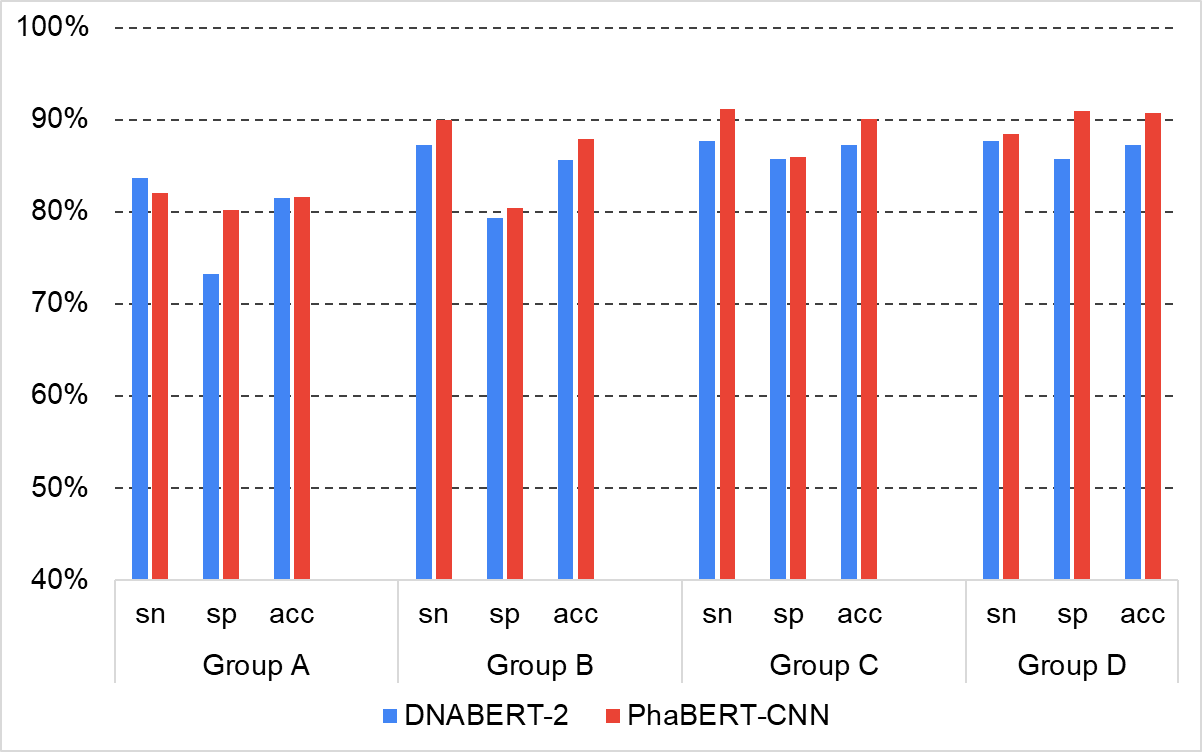
\includegraphics[width=0.8\linewidth]{imgs/dnabert2_vs_phabertcnn.png}
    \caption{So sánh hiệu suất giữa DNABERT-2 và PhaBERT-CNN}
    \label{fig:dnabert2_vs_phabertcnn}
\end{figure}

PhaBERT-CNN vượt trội hơn DNABERT-2 trên tất cả nhóm độ dài:

\begin{itemize}
    \item \textbf{Group A (100-400 bp)}: Accuracy 81.59\% vs 81.52\%, cải thiện specificity 6.90\% (80.15\% vs 73.25\%)
    \item \textbf{Group B (400-800 bp)}: Accuracy 87.91\% vs 85.56\%, cải thiện 2.35\%
    \item \textbf{Group C (800-1200 bp)}: Accuracy 90.01\% vs 87.25\%, cải thiện 2.76\%
    \item \textbf{Group D (1200-1800 bp)}: Accuracy 90.69\% vs 87.26\%, cải thiện 3.43\%
\end{itemize}

\textbf{Phân tích:} CNN và attention pooling giúp trích xuất đặc trưng task-specific hiệu quả hơn so với chỉ sử dụng [CLS] embedding của DNABERT-2.

\subsection{So sánh với các phương pháp tiên tiến}

\begin{table}[h]
\centering
\caption{So sánh hiệu suất trên 4 nhóm độ dài contig}
\label{tab:comparison}
\resizebox{\textwidth}{!}{%
\begin{tabular}{rccccc}
\toprule
\textbf{Method} & \textbf{Metric} & \textbf{Group A} & \textbf{Group B} & \textbf{Group C} & \textbf{Group D} \\
\midrule
\multirow{3}{*}{PhaBERT-CNN} & Sn & \textbf{82.00\%} & \textbf{89.91\%} & \textbf{91.12\%} & 88.47\% \\
 & Sp & 80.15\% & 80.44\% & 85.93\% & \textbf{90.95\%} \\
 & Acc & \textbf{81.59\%} & \textbf{87.91\%} & \textbf{90.01\%} & 90.69\% \\
\midrule
\multirow{3}{*}{PhaTYP} & Sn & 79.07\% & 86.74\% & 90.09\% & \textbf{92.29\%} \\
 & Sp & 78.77\% & \textbf{85.06\%} & \textbf{87.65\%} & 89.75\% \\
 & Acc & 78.92\% & 85.90\% & 88.87\% & \textbf{91.02\%} \\
\midrule
\multirow{3}{*}{DeePhage} & Sn & 80.09\% & 86.46\% & 89.17\% & 91.17\% \\
 & Sp & 71.79\% & 77.18\% & 80.13\% & 80.84\% \\
 & Acc & 78.07\% & 84.17\% & 87.40\% & 89.09\% \\
\midrule
\multirow{3}{*}{ProkBERT} & Sn & 80.65\% & 85.67\% & 83.61\% & 85.00\% \\
 & Sp & \textbf{80.80\%} & 84.15\% & 85.72\% & 83.68\% \\
 & Acc & 80.68\% & 85.35\% & 84.03\% & 84.73\% \\
\bottomrule
\end{tabular}%
}
\end{table}

\textbf{Kết quả chính:}

\begin{itemize}
    \item PhaBERT-CNN đạt accuracy cao nhất trên Groups A, B, C (81.59\%, 87.91\%, 90.01\%)
    \item PhaTYP tốt nhất trên Group D (91.02\%), nhưng PhaBERT-CNN cạnh tranh (90.69\%)
    \item PhaBERT-CNN cải thiện 0.91-5.98\% so với các baselines trên Groups A-C
    \item ProkBERT có performance stagnation, không cải thiện với longer contigs
\end{itemize}

\section{Thảo luận}

\subsection{Ưu điểm của PhaBERT-CNN}

\begin{enumerate}
    \item \textbf{Hiệu suất vượt trội trên short-medium contigs}: Đặc biệt quan trọng cho metagenomic analysis thực tế
    \item \textbf{Cân bằng sensitivity-specificity}: Duy trì balance tốt trên tất cả nhóm độ dài
    \item \textbf{Không phụ thuộc gene prediction}: Hoạt động trực tiếp trên DNA, khắc phục hạn chế của PhaTYP
    \item \textbf{Hybrid architecture}: Kết hợp global context (transformer) và local patterns (CNN)
\end{enumerate}

\subsection{Hạn chế}

\begin{itemize}
    \item Random undersampling có thể mất thông tin từ lớp đa số
    \item Computational cost cao hơn DeePhage do sử dụng transformer
    \item Hiệu suất trên Group D chưa vượt PhaTYP (nhưng cạnh tranh)
\end{itemize}

\subsection{Hướng cải thiện}

\begin{itemize}
    \item Thử các chiến lược xử lý imbalance khác (SMOTE, class weighting)
    \item Ablation studies chi tiết hơn về các thành phần kiến trúc
    \item Đánh giá trên real metagenomic datasets
    \item Tối ưu hóa inference speed cho deployment
\end{itemize}
        \caption{Dữ liệu ảnh chụp cột BTS04.}
        \label{fig:bts04}
    \end{figure} 

    \begin{figure}[H]
        \centering
        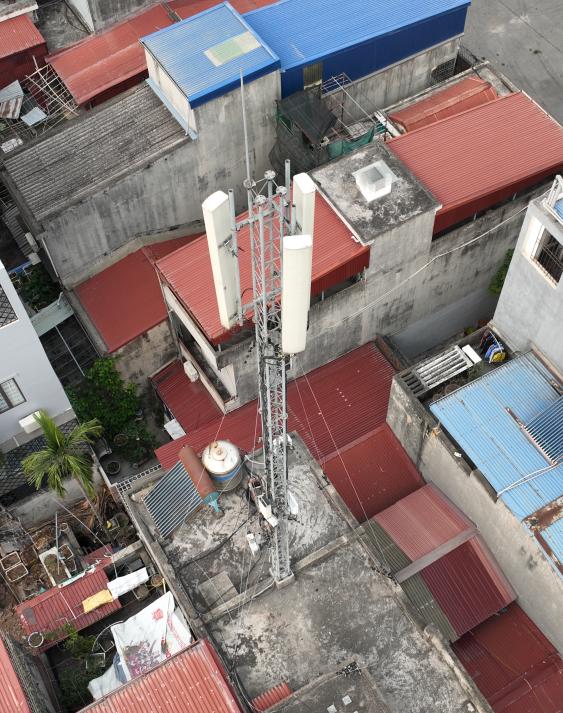
\includegraphics[width=0.45\linewidth]{figures/c4/bts5.png}
        \caption{Dữ liệu ảnh chụp cột BTS05.}
        \label{fig:bts05}
    \end{figure} 
    
    \subsection{Các phương pháp so sánh}
    \label{subsec:exp_baselines}
    \textbf{So sánh ước lượng camera pose}: So sánh độ chính xác camera pose trên các thí nghiệm bao gồm:
        \begin{itemize}
            \item Chỉ sử dụng SIFT
            \item Sử dụng SIFT kết hợp với lọc nhiễu
            \item Sử dụng SIFT kết hợp với ALIKED và phát hiện vùng ảnh ăng-ten
            \item Sử dụng SIFT kết hợp với ALIKED, phát hiện vùng ảnh ăng-ten và lọc nhiễu
        \end{itemize}
    \textbf{So sánh mô hình mây điểm 3D}: So sánh mô hình mây điểm 3D chi tiết từ camera pose tốt nhất của quy trình chỉ sử dụng SIFT và tốt nhất của quy trình kết hợp đặc trưng đề xuất với 2 thuật toán:
        \begin{itemize}
            \item MVS: Sử dụng thuật toán MVS trong nền tảng công cụ COLMAP.
            \item NeRF: Sử dụng mô hình nerfacto trong nền tảng công cụ Nerfstudio.
        \end{itemize}
    
    \subsection{Chỉ số đánh giá định lượng}
    \label{subsec:exp_metrics}
    \textbf{Lỗi chiếu ngược trung bình (MRE)}: được sử dụng để đánh giá độ chính xác của camera pose bằng cách đo lường sai số trung bình giữa các điểm 3D khi tái chiếu lên ảnh 2D so với các điểm đặc trưng trên ảnh đầu vào. Công thức tính MRE là: 
    \begin{equation}
        \text{MRE} = \frac{1}{N} \sum_{i=1}^N \|\pi(P_i, K, R, t) - p_i\|_2     
    \end{equation}
    trong đó \(P_i\) là điểm 3D, \(\pi\) là hàm tái chiếu sử dụng ma trận nội tại \(K\) và camera pose \((R, t)\), và \(p_i\) là tọa độ pixel của keypoint. Giá trị MRE càng thấp, mô hình 3D càng nhất quán với dữ liệu ảnh, phản ánh độ chính xác camera pose càng cao và chất lượng tái tạo càng tốt hơn.
    
    \textbf{Độ mượt bề mặt của đám mây điểm (PCS)}: được đo bằng cách tính độ biến thiên của các pháp tuyến hoặc độ cong tại các điểm, nhằm đánh giá mức độ nhiễu và tính liên tục của bề mặt. Độ đo này phản ánh chất lượng nội tại của mô hình 3D, chẳng hạn như mức độ gồ ghề do sai số camera pose gây ra. 

    Công thức tính độ mượt mà dựa trên độ cong trung bình được định nghĩa như sau:
    \begin{equation}
        \text{Smoothness} = \frac{1}{N} \sum_{i=1}^N \text{curvature}(p_i)
    \end{equation}

    trong đó \(\text{curvature}(p_i)\) là độ cong tại điểm \(p_i\), được ước lượng từ các điểm lân cận bằng thuật toán K láng giềng gần nhất. Một cách thay thế là tính độ biến thiên pháp tuyến, đo lường mức độ sai lệch của các pháp tuyến trong vùng lân cận so với pháp tuyến trung bình:
    \begin{equation}
        \text{Variance}_i = \frac{1}{k} \sum_{j \in \text{k-NN}(i)} \|\mathbf{n}_j - \overline{\mathbf{n}}\|_2
    \end{equation}

    với \(\mathbf{n}_j\) là pháp tuyến của điểm lân cận, \(\overline{\mathbf{n}}\) là pháp tuyến trung bình. Khi đó:
    \begin{equation}
        \text{Smoothness} = \frac{1}{N} \sum_{i=1}^N \text{Variance}_i
    \end{equation}

    Giá trị smoothness càng thấp, bề mặt càng mượt mà và ít nhiễu, cho thấy chất lượng mô hình tốt hơn.

    % \textbf{Độ lệch mặt phẳng (PE)}: Đo độ lệch của các điểm trên các bề mặt phẳng tái tạo so với mặt phẳng lý tưởng, đánh giá mức độ nhiễu trên bề mặt các thiết bị ăng-ten lắp đặt trên cột.
    
    % Công thức tính Planarity Error được định nghĩa như sau:
    % \[
    % \text{Planarity Error} = \frac{1}{N} \sum_{i=1}^N |a x_i + b y_i + c z_i + d|,
    % \]
    % trong đó \((a, b, c, d)\) là các tham số của mặt phẳng lý tưởng được ước lượng bằng thuật toán RANSAC, và \((x_i, y_i, z_i)\) là tọa độ của điểm \(p_i\) trong point cloud. Giá trị Planarity Error càng thấp, các điểm càng gần mặt phẳng lý tưởng, cho thấy mô hình có ít nhiễu và chất lượng cao hơn.
    
    \subsection{Môi trường thực thi}
    \label{subsec:exp_environment}
        Các thí nghiệm được cài đặt, triển khai trên môi trường bao gồm:
        \begin{itemize}
            % \item Phần cứng: RTX A4000 16GB VRAM, CPU 32 core, RAM 64GB.
            \item Phần cứng: RTX A4000 16GB VRAM, CPU 32 core, RAM 64GB.
            \item Phần mềm: COLMAP phiên bản 3.8, Nerfstudio phiên bản 1.0.3.
        \end{itemize}

    
\section{Đánh giá độ chính xác ước tính camera pose}
\label{sec:eval_pose}
Trong các đánh giá so sánh dưới đây, để đảm bảo tính khách quan thuật toán phát hiện điểm đặc trưng SIFT được cài đặt với tham số được đề cập trong bài báo \cite{Lowe04Distinctive}

\textbf{So sánh ảnh hưởng của số lượng điểm đặc trưng SIFT và bộ lọc điểm nhiễu dựa trên bản đồ độ sâu}
    Để đánh giá ảnh hưởng của số lượng điểm đặc trưng SIFT và bộ lọc nhiễu dựa trên bản đồ độ sâu lên độ chính xác của camera pose, quá trình đánh giá được thực hiện với 4 mức số lượng điểm đặc trưng: [2048, 4096, 8192, 16384]. Sau đó, với mỗi ảnh độ sâu tương đối (đã được chuyển về dạng grayscale) chúng tôi sử dụng 3 giá trị ngưỡng lọc THRESH = [30, 50, 100] để lọc các vị trí điểm đặc trưng được coi là nhiễu. 
    Từ kết quả Bảng \ref{tab:sift_comparison} cho thấy, việc áp dụng bộ lọc nhiễu dựa trên bản đồ độ sâu với ngưỡng THRESH phù hợp thực sự có thể giúp cải thiện độ chính xác camera pose. Nổi bật nhất là khi số lượng điểm đặc trưng lớn, đóng góp của bộ lọc nhiễu càng thêm rõ ràng.
    \begin{table}[ht]
        \centering
        \footnotesize
        \begin{tabular}{|l|c|c|c|c|c|}
        \hline
        \textbf{Phương pháp} & \textbf{BTS01} & \textbf{BTS02} & \textbf{BTS03} & \textbf{BTS04} & \textbf{BTS05} \\
        \hline
        SIFT-2K & 1.175 & 1.246 & 1.104 & \textbf{1.133} & \textbf{1.175} \\
        SIFT-2K+NF-30 & 1.184 & 1.238 & 1.105 & 1.142 & 1.178 \\
        SIFT-2K+NF-50 & \textbf{1.171} & \textbf{1.228} & \textbf{1.058} & 1.137 & \textbf{1.175} \\
        SIFT-2K+NF-100 & 1.177 & 1.251 & 1.119 & 1.130 & 1.183 \\
        \hline
        \end{tabular}
        \caption{So sánh sự ảnh hưởng của giá trị ngưỡng lọc điểm nhiễu dựa trên bản đồ độ sâu tương đối lên độ chính xác của camera pose với độ đo MRE (pixel).}
        \label{tab:sift_comparison}
    \end{table}

    \begin{table}[ht]
        \centering
        \footnotesize
        \begin{tabular}{|l|c|c|c|c|c|}
        \hline
        \textbf{Phương pháp} & \textbf{BTS01} & \textbf{BTS02} & \textbf{BTS03} & \textbf{BTS04} & \textbf{BTS05} \\
        \hline
        SIFT-2K & 1.175 & 1.246 & 1.104 & \textbf{1.133} & \textbf{1.175} \\
        SIFT-2K+NF-50 & \textbf{1.171} & \textbf{1.228} & \textbf{1.058} & 1.137 & \textbf{1.175}\\
        \hline
        SIFT-4K & \textbf{1.046} & 1.138 & 0.937 & 1.004 & 1.056 \\
        SIFT-4K+NF-50 & 1.050 & \textbf{1.122} & \textbf{0.894} & \textbf{1.001} & \textbf{1.054} \\
        \hline
        SIFT-8K & 0.899 & 0.961 & 0.782 & 0.874 & 0.902 \\
        SIFT-8K+NF-50 & \textbf{0.887} & \textbf{0.951} & \textbf{0.74} & \textbf{0.873} & \textbf{0.894} \\
        \hline
        SIFT-16K & 0.813 & 0.860 & 0.673 & 0.749 & 0.793 \\
        SIFT-16K+NF-50 & \textbf{0.788} & \textbf{0.839} & \textbf{0.639} & 0.749 & \textbf{0.788} \\
        \hline
        \end{tabular}
        \caption{So sánh độ hiệu quả của việc sử dụng bộ lọc điểm nhiễu dựa trên bản đồ độ sâu tương đối lên độ chính xác của camera pose với độ đo MRE (pixel).}
        \label{tab:sift_comparison}
    \end{table}

    
    	   	
\textbf{So sánh độ chính xác camera pose giữa phương pháp SfM truyền thống và phương pháp SfM lai ghép đề xuất}
Trong thực nghiệm này, chúng tôi tiến hành so sánh giá trị MRE của 3 phương pháp: SfM với thuật toán SfM truyền thống, SfM chỉ sử dụng ALIKED \cite{zhao2023aliked} và LightGlue \cite{lindenberger2023LightGlue}, và phương pháp SfM lai ghép đề xuất. Thực nghiệm được tiến hành với 3 giá trị tổng số lượng điểm đặc trưng được trích xuất lần lượt là 4096, 8192, 16384 (điểm).
    \begin{table}[H]
    \centering
    \footnotesize
    \begin{tabular}{|l|c|c|c|c|c|}
    \hline
    \textbf{Phương pháp} & \textbf{BTS01} & \textbf{BTS02} & \textbf{BTS03} & \textbf{BTS04} & \textbf{BTS05} \\
    \hline
    SIFT-4K & 1.046 & 1.138 & 0.937 & 1.004 & 1.056 \\
    ALIKED-4K & 0.756 & 0.892 & 0.704 & 0.671 & 0.798 \\
    SIFT-2K+ALIKED-2K+NF & \textbf{0.606} & \textbf{0.682} & \textbf{0.578} & \textbf{0.577} & \textbf{0.598} \\
    \hline
    SIFT-8K & 0.899 & 0.961 & 0.782 & 0.874 & 0.902 \\
    ALIKED-8K & 0.711 & 0.755 & 0.727 & 0.680 & 0.712 \\
    SIFT-4K+ALIKED-2K+NF & 0.615 & 0.702 & 0.574 & 0.565 & 0.636 \\
    SIFT-4K+ALIKED-4K+NF & \textbf{0.558} & \textbf{0.615} & \textbf{0.557} & \textbf{0.514} & \textbf{0.588} \\
    \hline
    SIFT-16K & 0.813 & 0.860 & 0.673 & 0.749 & 0.793\\
    ALIKED-16K & 0.683 & 0.721 & 0.714 & 0.677 & 0.736 \\
    SIFT-8K+ALIKED-2K+NF & 0.651 & 0.726 & 0.652 & 0.629 & 0.682 \\
    SIFT-8K+ALIKED-4K+NF & 0.556 & 0.62 & \textbf{0.539} & 0.538 & 0.609 \\
    SIFT-8K+ALIKED-8K+NF & \textbf{0.544} & \textbf{0.579} & 0.545 & \textbf{0.519} & \textbf{0.585} \\ 
    \hline
    \end{tabular}
    \caption{So sánh giá trị MRE (px) khi tính toán camera pose giữa giải pháp SfM truyền thống và giải pháp SfM lai ghép đề xuất, các kết quả MRE trên đều đi kèm với tỉ lệ ảnh được đăng ký khi thực hiện SfM là 100\%.}
    \label{tab:comparison}
    \end{table}

    Từ kết quả thực nghiệm Bảng \ref{tab:comparison}, phương pháp SfM lai ghép (kết hợp SIFT và ALIKED với kỹ thuật lọc nhiễu) cho thấy hiệu quả vượt trội so với các phương pháp SfM truyền thống (SIFT) hoặc phương pháp SfM sử dụng ALIKED đơn lẻ, với giá trị MRE thấp hơn đáng kể trên tất cả các tập dữ liệu. Đặc biệt, với cấu hình SIFT-8K+ALIKED-8K+NF đạt MRE thấp nhất, từ 0.519 đến 0.585 px, chứng tỏ sự cải thiện rõ rệt khi bổ sung các điểm đặc trưng, các cặp so khớp tập trung vào vùng cột với ALIKED và LightGlue, kết hợp với SIFT làm đầu vào cho bước tái tạo dần dần (mục \ref{subsec:incremental_reconstruction}). Thậm chí, với tổng số lượng điểm đặc trưng khi trích xuất khoảng 4096 điểm, thì SIFT-2K+ALIKED-2K+NF đã có kết quả MRE thấp hơn đáng kế so với SIFT-16K. Điều này càng làm nổi bật độ hiệu quả của phương pháp SfM đề xuất. Bên cạnh đó, thí nghiệm SIFT-8K+ALIKED-2K+NF, SIFT-8K+ALIKED-4K+NF, SIFT-8K+ALIKED-8K+NF cho thấy khi tăng số lượng điểm đặc trưng và các cặp so khớp ALIKED, kết quả MRE cũng gần như giảm dần trên tất cả các tập dữ liệu chứng tỏ việc kết hợp ALIKED giúp phát hiện và bổ sung những đặc trưng quan trọng, tốt khác mà SIFT không phát hiện được, giúp cải thiện độ chính xác tính toán ước tính camera pose. Hình \ref{fig:comparison_keypoints} cho thấy, việc sử dụng ALIKED đã giúp phát hiện thêm các điểm đặc trưng quan trọng tập trung vào vùng thân và xung quanh chân cột hơn là chỉ sử dụng thuật toán trích xuất đặc trưng SIFT.

    Việc cho kết quả tốt hơn, cho thấy việc keypoints 

    \begin{figure}[H]
        \centering
        \begin{subfigure}[b]{0.45\textwidth}
            \centering
            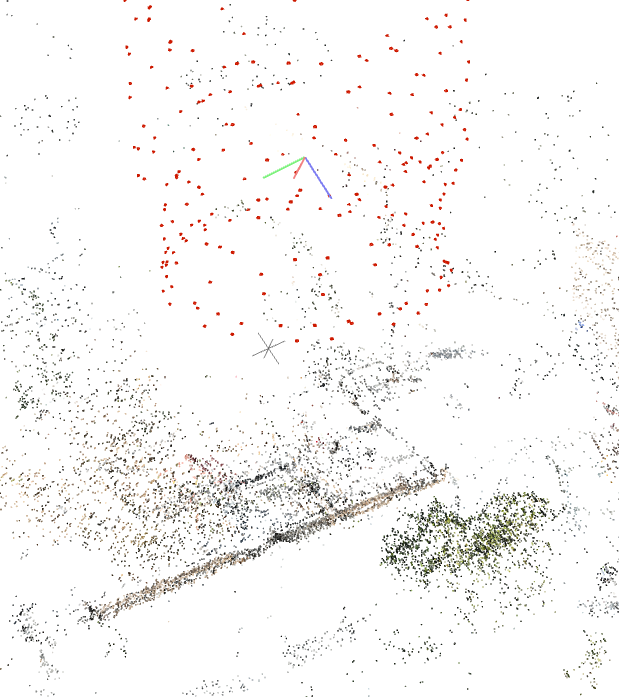
\includegraphics[width=0.85\linewidth]{figures/c4/colmap_sfm.png}
            % \caption{Ảnh 1}
            \end{subfigure}
        \hfill
        \begin{subfigure}[b]{0.45\textwidth}
            \centering
            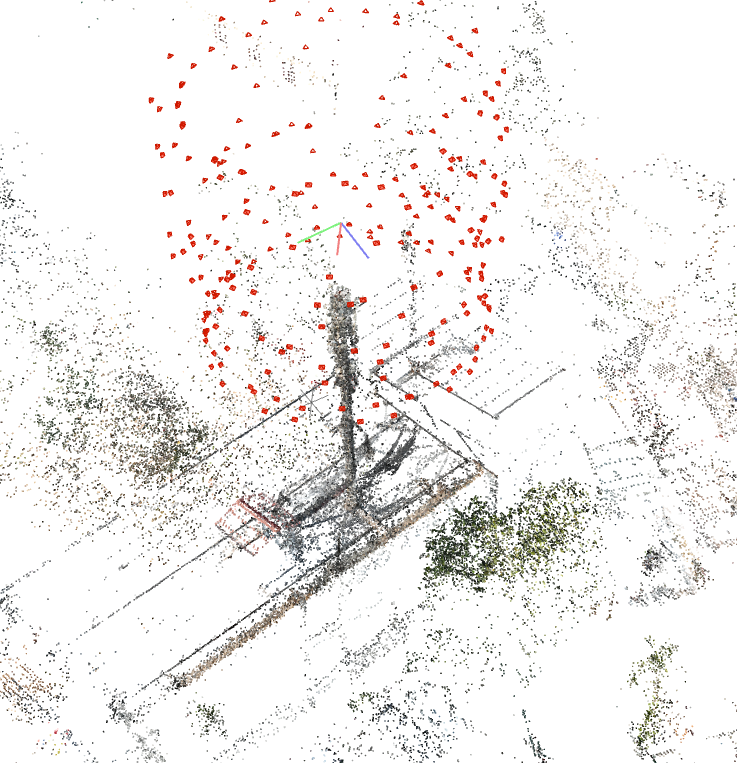
\includegraphics[width=0.85\linewidth]{figures/c4/colmap_deep_keys.png}
            % \caption{Ảnh 2}
            \end{subfigure}
        \caption{So sánh mức độ tập trung keypoints vào cột ăng-ten, ảnh bên trái là giải pháp SfM truyền thống, ảnh bên phải là giải pháp SfM lai ghép để xuất, kết quả được dựng từ SIFT-16K và SIFT-8K+ALIKED-8K+NF.}
        \label{fig:comparison_keypoints}
    \end{figure}
    
\textbf{So sánh thời gian thực thi thuật toán}

Chúng tôi thực hiện thí nghiệm đo thời gian thực thi thuật toán trung bình trên 5 tập dữ liệu thực tế, giữa phương pháp SfM truyền thống và phương pháp SfM đề xuất. Mục tiêu của thí nghiệm này là so sánh thời gian thực thi trung bình giữa các phương pháp với điều kiện 1 tập dữ liệu có trung bình 350 ảnh và trích xuất số lượng điểm đặc trưng bằng nhau.

Từ kết quả Bảng \ref{tab:time} có thể thấy rằng thời gian khi trích xuất cùng số lượng điểm đặc trưng thì phương pháp SfM lai ghép đề xuất có thời gian thực thi tăng đáng kể so với phương pháp truyền thống. Nguyên nhân là do quá trình trích xuất và so khớp của ALIKED chậm hơn SIFT đáng kể dẫn tới thời gian bị tăng lên rõ rệt.
    \begin{table}[H]
    \centering
    \footnotesize
    \begin{tabular}{|l|c|}
    \hline
    \textbf{Phương pháp} & \textbf{Thời gian (Xấp xỉ)} \\
    \hline
    SIFT-4K & 18 \\
    ALIKED-4K & 20 \\ %30m
    SIFT-2K+ALIKED-2K+NF & 23  \\
    \hline
    SIFT-8K &  38 \\
    ALIKED-8K &  55 \\ % 120m
    SIFT-4K+ALIKED-2K+NF & 43 \\
    SIFT-4K+ALIKED-4K+NF & 61  \\
    \hline
    SIFT-16K & 65\\
    ALIKED-16K & 155  \\ 
    SIFT-8K+ALIKED-2K+NF & 48 \\
    SIFT-8K+ALIKED-4K+NF & 76  \\
    SIFT-8K+ALIKED-8K+NF & 95 \\ 
    \hline
    \end{tabular}
    \caption{So sánh thời gian (phút) thực thi thuật toán trung bình giữa giải pháp SfM truyền thống và giải pháp SfM lai ghép đề xuất trên 5 tập ảnh thử nghiệm.}
    \label{tab:time}
    \end{table}
% Dựa trên bảng số liệu về giá trị MRE (đơn vị: px) khi tính toán camera pose trên 5 tập dữ liệu cột ăng-ten thực tế (BTS01 đến BTS05), có thể đưa ra một số nhận xét khoa học như sau. Phương pháp \textbf{SIFT+ALIKED+NF} cho thấy hiệu suất vượt trội nhất với giá trị MRE thấp nhất trên tất cả các tập dữ liệu, dao động từ 0.773147 (BTS05) đến 0.944814 (BTS02), thể hiện độ chính xác cao và độ nhất quán tốt khi tái chiếu các điểm 3D lên ảnh 2D. Trong khi đó, phương pháp chỉ sử dụng \textbf{SIFT} truyền thống có giá trị MRE cao hơn đáng kể, lần lượt dao động từ 0.937670 đến 1.138319, cho thấy sai số tái chiếu lớn hơn và hiệu quả kém hơn. Kết quả này cho thấy việc kết hợp SIFT, ALIKED và lọc đặc trưng nhiễu ở xa không chỉ giảm thiểu nhiễu mà còn tăng cường độ chính xác trong tính toán camera pose, đặc biệt trong các ứng dụng thực tế như tái tạo 3D cột ăng-ten.

\section{Đánh giá sự ảnh hưởng của camera pose tới chất lượng tái tạo mây điểm 3D chi tiết}
\label{sec:eval_dense}
     % Luận văn đánh giá sự ảnh hưởng của độ chính xác camera pose lên NeRF thông qua 2 độ đo: Độ lệch mặt phẳng (PE) và Độ mượt mà của đám mây điểm (PCS).
     % \begin{itemize}
     %     \item \textbf{Độ lệch mặt phẳng:} Được thực hiện bằng cách cắt bề mặt 3 thiết bị ăng-ten từ mô hình 3D chi tiết. Sau đó, sử dụng thư viện open3d để xấp xỉ mặt phẳng bề mặt cho mỗi ăng-ten. Cuối cùng, tính toán giá trị PE cho mỗi bề mặt được cắt và tính toán giá trị trung bình.
     %     \item \textbf{Độ mượt mà của đám mây điểm:} Được thực hiện bằng cách cắt hoàn chỉnh 3 thiết bị ăng-ten từ mô hình 3D chi tiết. Sau đó, sử dụng thư viện open3d để ước lượng vector pháp tuyến cho mỗi điểm trong mây điểm thiết bị ăng-ten. Tiếp theo, thực hiện duyệt qua mây điểm, tại mỗi điểm, xác định tập các điểm lân cận của nó và tính toán độ biến thiên vector pháp tuyến của tập điểm lân cận đó. Cuối cùng là tính giá trị trung bình cho toàn bộ điểm trên bề mặt thiết bị.
     % \end{itemize}
     Luận văn đánh giá sự ảnh hưởng của độ chính xác camera pose lên chất lượng mô hình mây điểm 3D tái tạo thông qua độ đo PCS. Chúng tôi sử dụng 3 tập dữ liệu BTS01, BTS03 và BTS05 đặc trưng cho 3 loại cột phổ biến trong lĩnh vực viễn thông để tiến hành đánh giá. Khi tiến hành thử nghiệm, chúng tôi lựa chọn camera pose tốt nhất từ 2 phương pháp SfM truyền thống (SIFT-16K) và SfM đề xuất (SIFT-8K+ALIKED-8K+NF) để thực hiện tái tạo mô hình mây điểm 3D chi tiết. Để tính chỉ số PCS, chúng tôi thực hiện cắt riêng 3 thiết bị ăng-ten được lắp đặt trên cột của từng mô hình. Sau đó, sử dụng thư viện open3d để ước lượng vector pháp tuyến cho mỗi điểm trong mây điểm thiết bị ăng-ten. Tiếp theo, thực hiện duyệt qua mây điểm, tại mỗi điểm, xác định tập các điểm lân cận của nó và tính toán độ biến thiên vector pháp tuyến của tập điểm lân cận đó. Cuối cùng là tính giá trị trung bình cho toàn bộ điểm trên bề mặt thiết bị.

     
    \subsection{Ảnh hưởng của độ chính xác camera pose lên chất lượng tái tạo mây điểm 3D chi tiết của MVS}
    \label{subsec:eval_mvs_impact}
        \begin{table}[H]
            \centering
            \footnotesize
            \begin{tabular}{|l|l|c|c|c|}
            \hline
            \textbf{Dữ liệu} & \textbf{Phương pháp} & \textbf{Ăng-ten 1} & \textbf{Ăng-ten 2} & \textbf{Ăng-ten 3} \\
            \hline
            BTS01 & SIFT-16K & 0.337 & 0.271 & 0.379 \\
                  & SIFT-8K+ALIKED-8K+NF & \textbf{0.308} & \textbf{0.269} & \textbf{0.316} \\
            \hline
            BTS03 & SIFT-16K & 0.311 & 0.350 & 0.327 \\
                  & SIFT-8K+ALIKED-8K+NF & \textbf{0.161} & \textbf{0.157} & \textbf{0.168} \\
            \hline
            BTS05 & SIFT-16K & 0.392 & 0.365 & 0.332 \\
                  & SIFT-8K+ALIKED-8K+NF & \textbf{0.326} & \textbf{0.296} & \textbf{0.231}\\
            \hline
            \end{tabular}
            \caption{So sánh chỉ số PCS của mô hình mây điểm tái tạo từ MVS với 2 đầu vào từ 2 phương pháp: SfM truyền thống và SfM đề xuất.}
            \label{tab:Smoothness_comparison_mvs}
        \end{table}
    Kết quả của thực nghiệm được tổng hợp tại Bảng \ref{tab:Smoothness_comparison_mvs} cho thấy rằng, việc cải thiện độ chính xác ước tính camera pose cũng đồng thời giúp cải thiện độ chính xác hình học của mô hình mây điểm 3D tái tạo sử dụng MVS. Trên 3 tập dữ liệu thử nghiệm, giá trị PCS của phương pháp SIFT-8K+ALIKED-8K+NF đều giảm so với phương pháp SIFT-16K. Thật vây, thông qua các hình ảnh so sánh biểu diễn điểm 3D của các thiết bị tại Hình \ref{fig:mvs_device_bts01}, Hình \ref{fig:mvs_device_bts03} và Hình \ref{fig:mvs_device_bts05} cho thấy, mây điểm 3D thiết bị được tái tạo với đầu vào từ SIFT-8K+ALIKED-8K+NF có độ mịn, phẳng và ít nhiễu hơn so với biểu diễn mây điểm 3D thiết bị với đầu vào từ SIFT-16K.
    
    \begin{figure}[htbp]
        \centering
    
        % Cặp 1
        \begin{subfigure}[b]{0.3\textwidth}
            \centering
            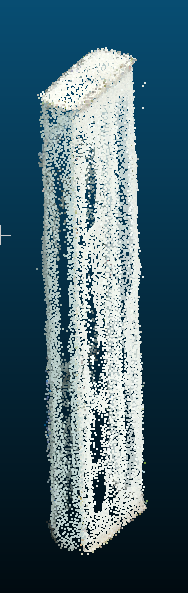
\includegraphics[width=0.45\textwidth]{figures/c4/sift_1_a1.png}
            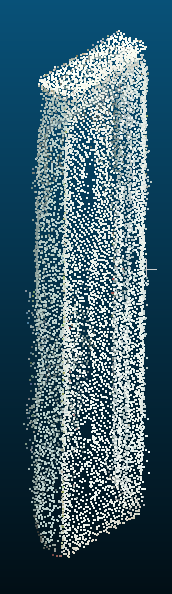
\includegraphics[width=0.41\textwidth]{figures/c4/deep_1_a1.png}
            \caption{Ăng-ten 1}
        \end{subfigure}
        \hfill
        % Cặp 2
        \begin{subfigure}[b]{0.3\textwidth}
            \centering
            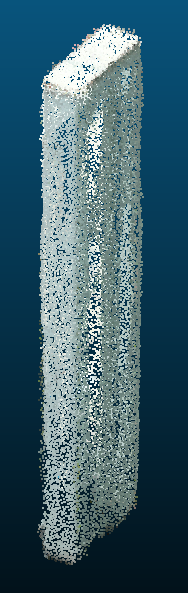
\includegraphics[width=0.45\textwidth]{figures/c4/sift_1_a2.png}
            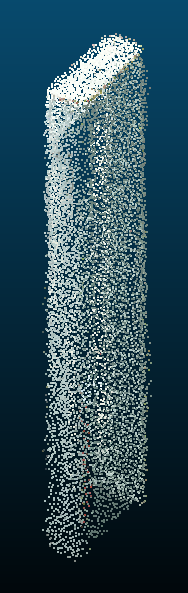
\includegraphics[width=0.45\textwidth]{figures/c4/deep_1_a2.png}
            \caption{Ăng-ten 2}
        \end{subfigure}
        \hfill
        % Cặp 3
        \begin{subfigure}[b]{0.3\textwidth}
            \centering
            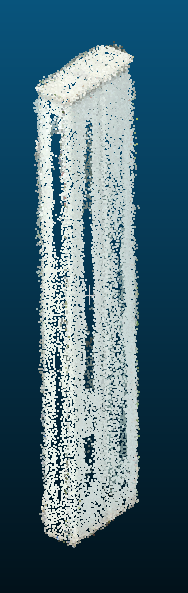
\includegraphics[width=0.45\textwidth]{figures/c4/sift_1_a3.png}
            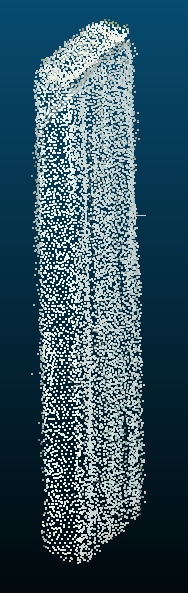
\includegraphics[width=0.45\textwidth]{figures/c4/deep_1_a3.png}
            \caption{Ăng-ten 3}
        \end{subfigure}
    
        \caption{So sánh biểu diễn mây điểm 3D của từng thiết bị ăng-ten trạm BTS01 được tái tạo bằng MVS. Trong mỗi cặp ảnh, ảnh bên trái là kết quả của SIFT-16K, bên phải là kết quả của SIFT-8K+ALIKED-8K+NF}
        \label{fig:mvs_device_bts01}
    \end{figure}

    \begin{figure}[htbp]
        \centering
    
        % Cặp 1
        \begin{subfigure}[b]{0.3\textwidth}
            \centering
            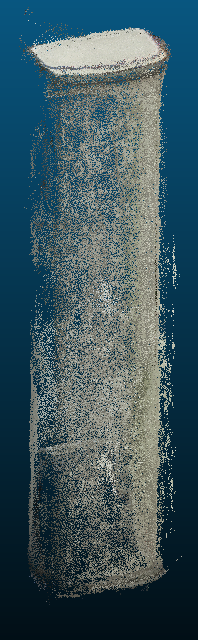
\includegraphics[width=0.45\textwidth]{figures/c4/sift_3_a1.png}
            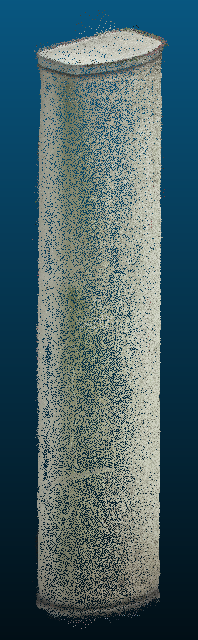
\includegraphics[width=0.45\textwidth]{figures/c4/deep_3_a1.png}
            \caption{Ăng-ten 1}
        \end{subfigure}
        \hfill
        % Cặp 2
        \begin{subfigure}[b]{0.3\textwidth}
            \centering
            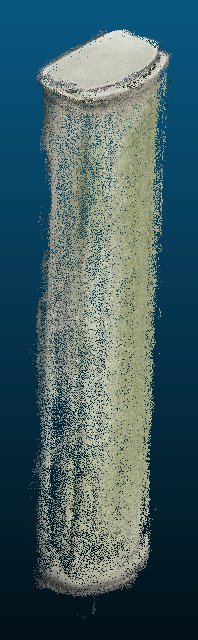
\includegraphics[width=0.45\textwidth]{figures/c4/sift_3_a2.png}
            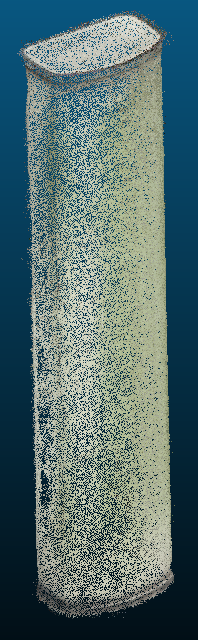
\includegraphics[width=0.45\textwidth]{figures/c4/deep_3_a2.png}
            \caption{Ăng-ten 2}
        \end{subfigure}
        \hfill
        % Cặp 3
        \begin{subfigure}[b]{0.3\textwidth}
            \centering
            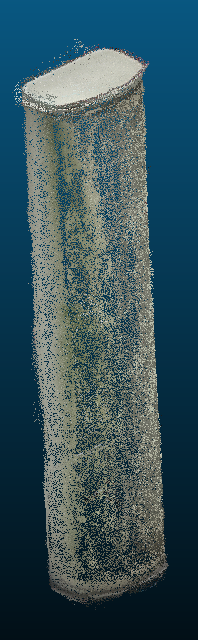
\includegraphics[width=0.45\textwidth]{figures/c4/sift_3_a3.png}
            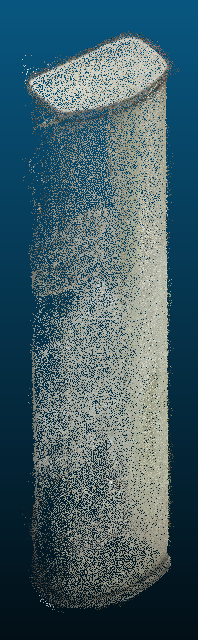
\includegraphics[width=0.45\textwidth]{figures/c4/deep_3_a3.png}
            \caption{Ăng-ten 3}
        \end{subfigure}
    
        \caption{So sánh biểu diễn mây điểm 3D của từng thiết bị ăng-ten trạm BTS03 được tái tạo bằng MVS. Trong mỗi cặp ảnh, ảnh bên trái là kết quả của SIFT-16K, bên phải là kết quả của SIFT-8K+ALIKED-8K+NF}
        \label{fig:mvs_device_bts03}
    \end{figure}

    \begin{figure}[htbp]
        \centering
    
        % Cặp 1
        \begin{subfigure}[b]{0.3\textwidth}
            \centering
            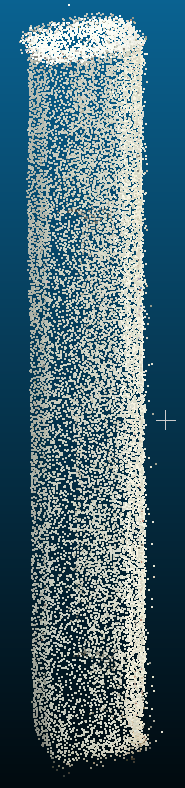
\includegraphics[width=0.45\textwidth]{figures/c4/sift_5_a1.png}
            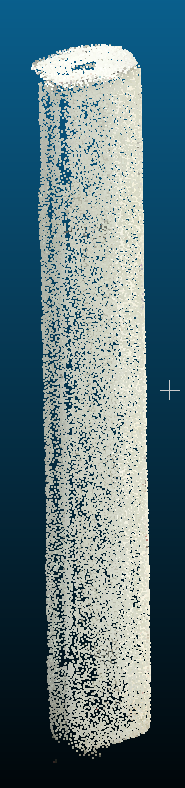
\includegraphics[width=0.45\textwidth]{figures/c4/deep_5_a1.png}
            \caption{Ăng-ten 1}
        \end{subfigure}
        \hfill
        % Cặp 2
        \begin{subfigure}[b]{0.3\textwidth}
            \centering
            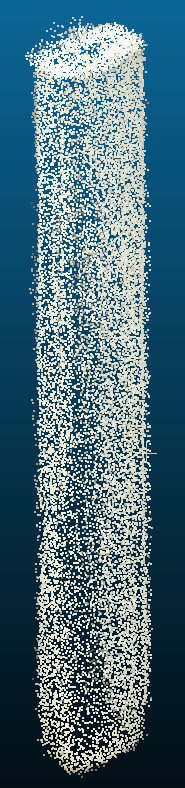
\includegraphics[width=0.45\textwidth]{figures/c4/sift_5_a2.png}
            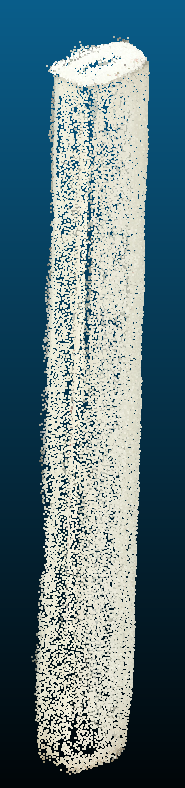
\includegraphics[width=0.45\textwidth]{figures/c4/deep_5_a2.png}
            \caption{Ăng-ten 2}
        \end{subfigure}
        \hfill
        % Cặp 3
        \begin{subfigure}[b]{0.3\textwidth}
            \centering
            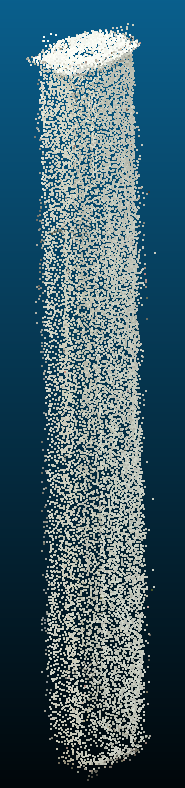
\includegraphics[width=0.45\textwidth]{figures/c4/sift_5_a3.png}
            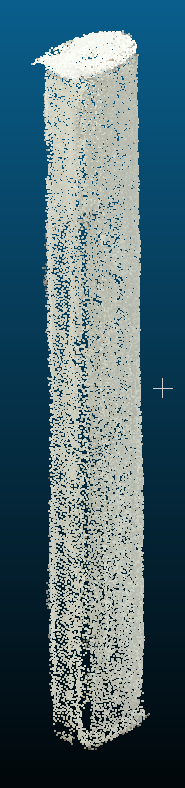
\includegraphics[width=0.45\textwidth]{figures/c4/deep_5_a3.png}
            \caption{Ăng-ten 3}
        \end{subfigure}
    
        \caption{So sánh biểu diễn mây điểm 3D của từng thiết bị ăng-ten trạm BTS05 được tái tạo bằng MVS. Trong mỗi cặp ảnh, ảnh bên trái là kết quả của SIFT-16K, bên phải là kết quả của SIFT-8K+ALIKED-8K+NF}
        \label{fig:mvs_device_bts05}
    \end{figure}
    
    \subsection{Ảnh hưởng của độ chính xác camera pose lên chất lượng tái tạo mây điểm 3D chi tiết của NeRF}
    
     \label{subsec:eval_nerf_impact}
        \begin{table}[H]
            \centering
            \footnotesize
            \begin{tabular}{|l|l|c|c|c|}
            \hline
            \textbf{Dữ liệu} & \textbf{Phương pháp} & \textbf{Ăng-ten 1} & \textbf{Ăng-ten 2} & \textbf{Ăng-ten 3} \\
            \hline
            BTS01 & SIFT-16K & 0.775 & 0.783 & 0.728 \\
                  & SIFT-8K+ALIKED-8K+NF & \textbf{0.757} & \textbf{0.761} & \textbf{0.725}\\
            \hline
            BTS03 & SIFT-16K & 0.738 & 0.658 & 0.672 \\
                  & SIFT-8K+ALIKED-8K+NF & \textbf{0.724} & \textbf{0.637} &  \textbf{0.648}\\
            \hline
            BTS05 & SIFT-16K & 0.732 & 0.747 & 0.755 \\
                  & SIFT-8K+ALIKED-8K+NF & \textbf{0.706} & \textbf{0.730} & \textbf{0.735} \\
            \hline
            \end{tabular}
            \caption{So sánh chỉ số PCS của mô hình mây điểm tái tạo từ Nerfacto với 2 đầu vào từ 2 phương pháp: SfM truyền thống và SfM đề xuất.}
            \label{tab:Smoothness_comparison_nerf}
        \end{table}
    
    Từ Bảng \ref{tab:Smoothness_comparison_nerf} cho thấy kết quả tương đồng với thực nghiệm \ref{subsec:eval_mvs_impact}. Có thể thấy, chỉ số PCS của mô hình mây điểm 3D tương ứng với phương pháp lai ghép SIFT-8K+ALIKED-8K+NF giảm trung bình xấp xỉ 3\% so với phương pháp truyền thống chỉ sử dụng SIFT (SIFT-16K). Rõ ràng, kết quả của Bảng \ref{tab:Smoothness_comparison_mvs} và \ref{tab:Smoothness_comparison_nerf} chứng tỏ việc cải thiện độ chính xác ước tính camera pose cũng làm tăng độ chính xác của đám mây điểm chi tiết sau khi tái tạo.

    \begin{figure}[htbp]
        \centering
    
        % Cặp 1
        \begin{subfigure}[b]{0.3\textwidth}
            \centering
            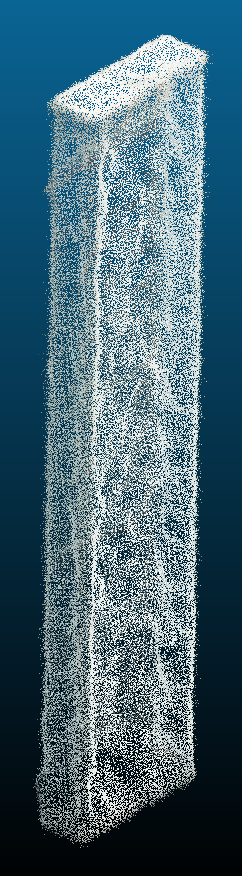
\includegraphics[width=0.45\textwidth]{figures/c4/nerf_sift_1_a1.png}
            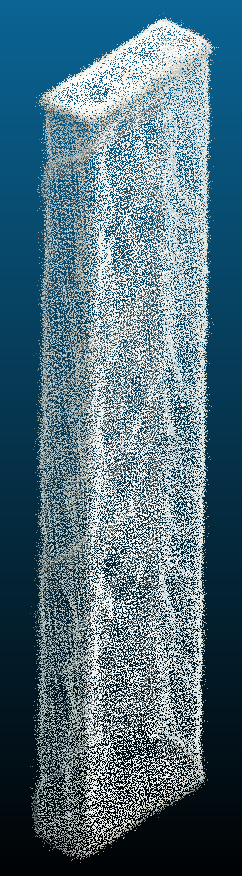
\includegraphics[width=0.45\textwidth]{figures/c4/nerf_deep_1_a1.png}
            \caption{Ăng-ten 1}
        \end{subfigure}
        \hfill
        % Cặp 2
        \begin{subfigure}[b]{0.3\textwidth}
            \centering
            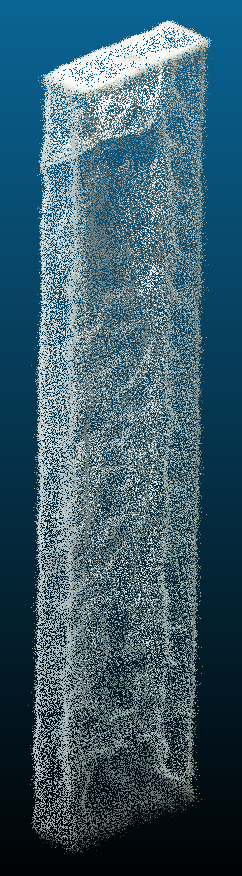
\includegraphics[width=0.45\textwidth]{figures/c4/nerf_sift_1_a2.png}
            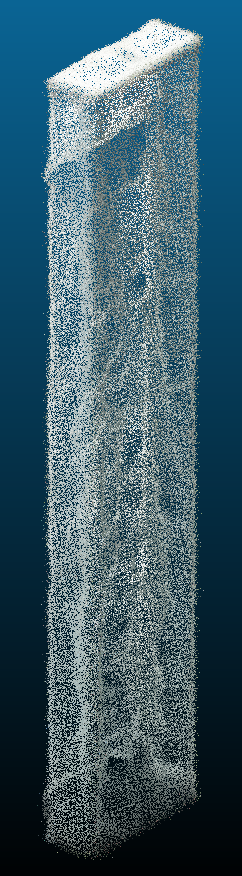
\includegraphics[width=0.45\textwidth]{figures/c4/nerf_deep_1_a2.png}
            \caption{Ăng-ten 2}
        \end{subfigure}
        \hfill
        % Cặp 3
        \begin{subfigure}[b]{0.3\textwidth}
            \centering
            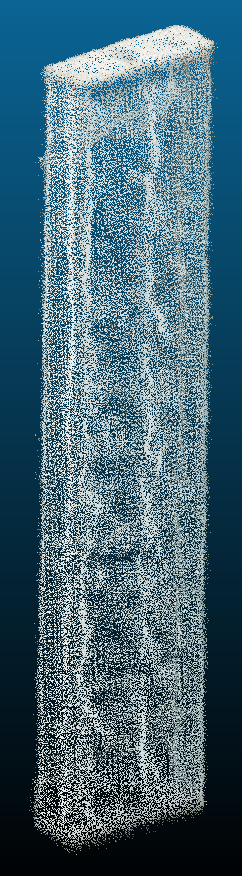
\includegraphics[width=0.45\textwidth]{figures/c4/nerf_sift_1_a3.png}
            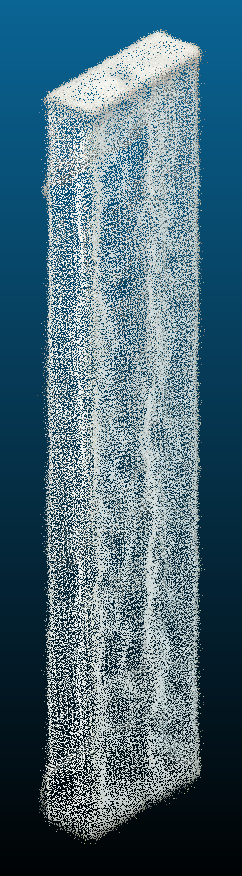
\includegraphics[width=0.45\textwidth]{figures/c4/nerf_deep_1_a3.png}
            \caption{Ăng-ten 3}
        \end{subfigure}
    
        \caption{So sánh biểu diễn mây điểm 3D của từng thiết bị ăng-ten trạm BTS01 được tái tạo bằng Nerfacto. Trong mỗi cặp ảnh, ảnh bên trái là kết quả của SIFT-16K, bên phải là kết quả của SIFT-8K+ALIKED-8K+NF}
        \label{fig:nerf_device_bts01}
    \end{figure}

    \begin{figure}[htbp]
        \centering
    
        % Cặp 1
        \begin{subfigure}[b]{0.3\textwidth}
            \centering
            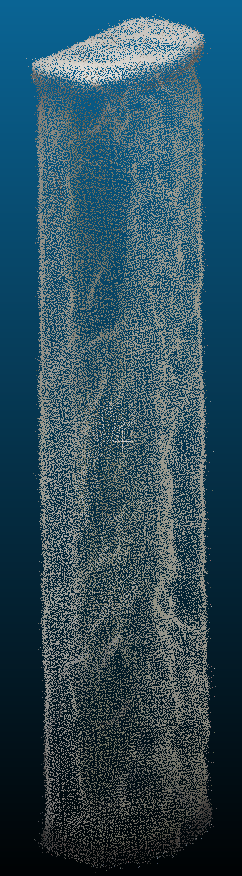
\includegraphics[width=0.45\textwidth]{figures/c4/nerf_sift_3_a1.png}
            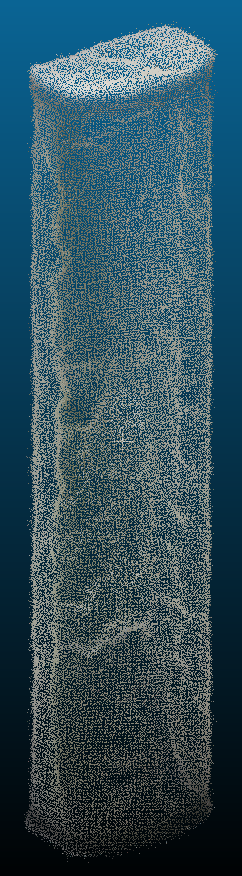
\includegraphics[width=0.45\textwidth]{figures/c4/nerf_deep_3_a1.png}
            \caption{Ăng-ten 1}
        \end{subfigure}
        \hfill
        % Cặp 2
        \begin{subfigure}[b]{0.3\textwidth}
            \centering
            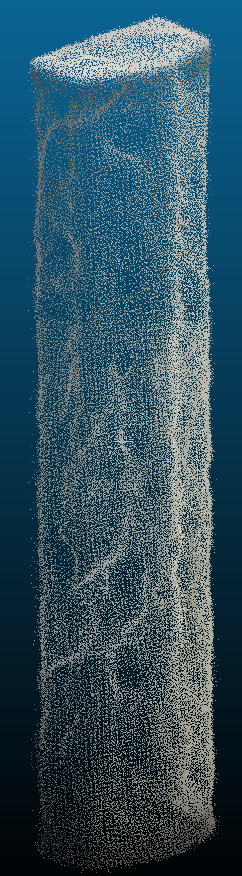
\includegraphics[width=0.45\textwidth]{figures/c4/nerf_sift_3_a2.png}
            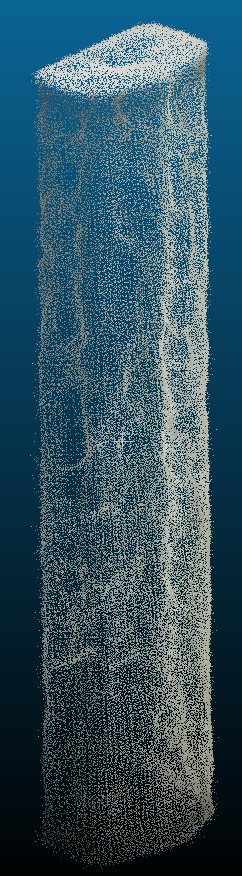
\includegraphics[width=0.45\textwidth]{figures/c4/nerf_deep_3_a2.png}
            \caption{Ăng-ten 2}
        \end{subfigure}
        \hfill
        % Cặp 3
        \begin{subfigure}[b]{0.3\textwidth}
            \centering
            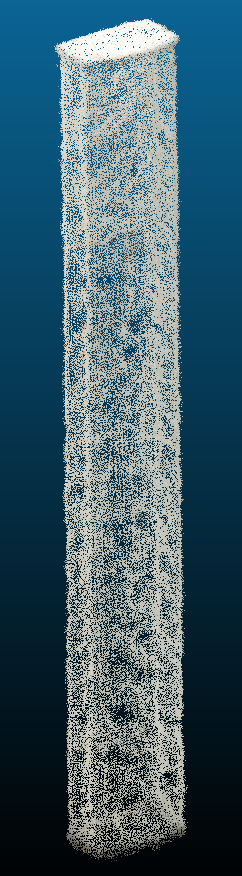
\includegraphics[width=0.45\textwidth]{figures/c4/nerf_sift_5_a3.png}
            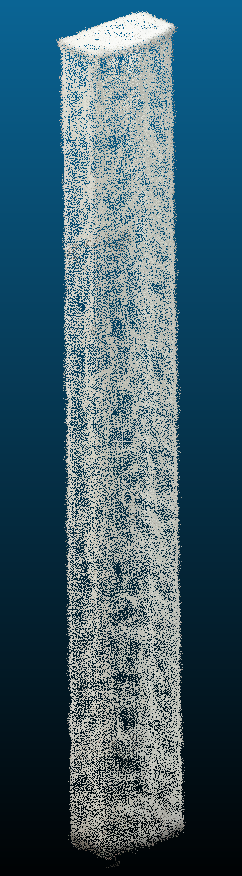
\includegraphics[width=0.45\textwidth]{figures/c4/nerf_deep_5_a3.png}
            \caption{Ăng-ten 3}
        \end{subfigure}
    
        \caption{So sánh biểu diễn mây điểm 3D của từng thiết bị ăng-ten trạm BTS03 được tái tạo bằng Nerfacto. Trong mỗi cặp ảnh, ảnh bên trái là kết quả của SIFT-16K, bên phải là kết quả của SIFT-8K+ALIKED-8K+NF}
        \label{fig:nerf_device_bts03}
    \end{figure}

    \begin{figure}[htbp]
        \centering
    
        % Cặp 1
        \begin{subfigure}[b]{0.3\textwidth}
            \centering
            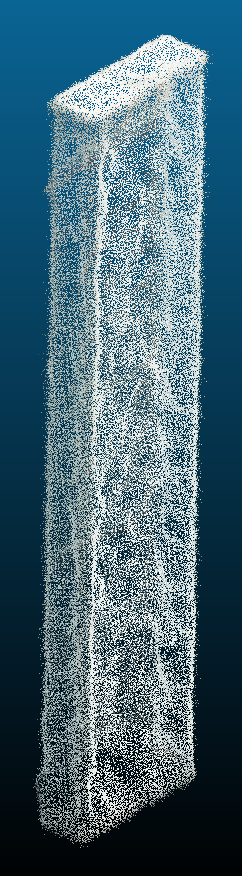
\includegraphics[width=0.45\textwidth]{figures/c4/nerf_sift_1_a1.png}
            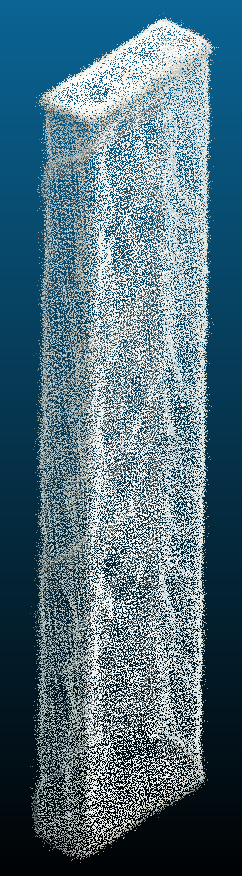
\includegraphics[width=0.45\textwidth]{figures/c4/nerf_deep_1_a1.png}
            \caption{Ăng-ten 1}
        \end{subfigure}
        \hfill
        % Cặp 2
        \begin{subfigure}[b]{0.3\textwidth}
            \centering
            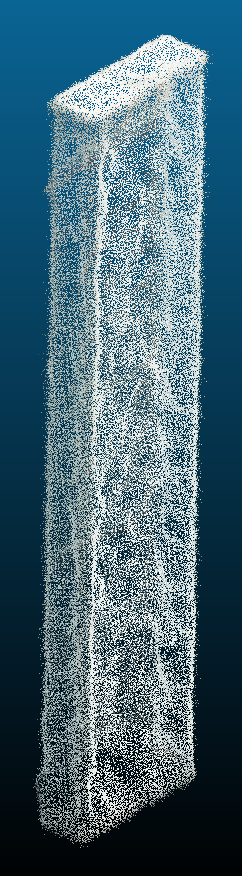
\includegraphics[width=0.45\textwidth]{figures/c4/nerf_sift_1_a1.png}
            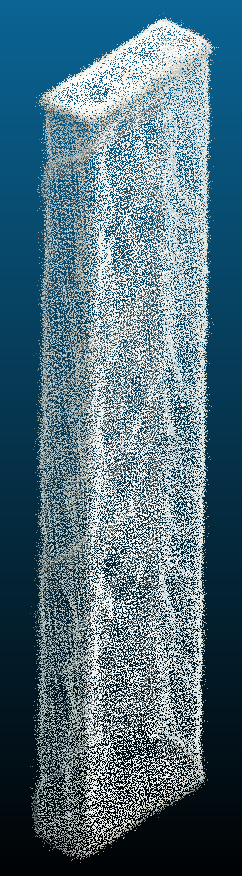
\includegraphics[width=0.45\textwidth]{figures/c4/nerf_deep_1_a1.png}
            \caption{Ăng-ten 2}
        \end{subfigure}
        \hfill
        % Cặp 3
        \begin{subfigure}[b]{0.3\textwidth}
            \centering
            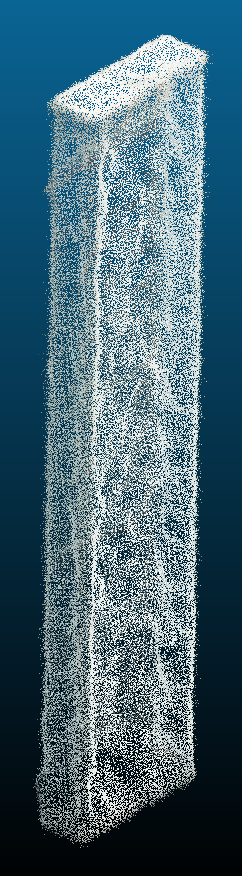
\includegraphics[width=0.45\textwidth]{figures/c4/nerf_sift_1_a1.png}
            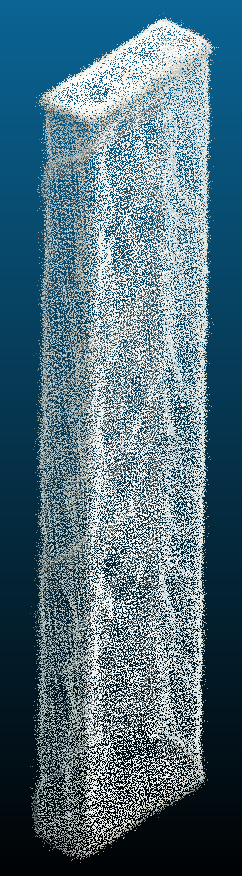
\includegraphics[width=0.45\textwidth]{figures/c4/nerf_deep_1_a1.png}
            \caption{Ăng-ten 3}
        \end{subfigure}
    
        \caption{So sánh biểu diễn mây điểm 3D của từng thiết bị ăng-ten trạm BTS05 được tái tạo bằng Nerfacto. Trong mỗi cặp ảnh, ảnh bên trái là kết quả của SIFT-16K, bên phải là kết quả của SIFT-8K+ALIKED-8K+NF}
        \label{fig:nerf_device_bts05}
    \end{figure}
    Từ Hình \ref{fig:nerf_device_bts01}, Hình \ref{fig:nerf_device_bts03}, Hình \ref{fig:nerf_device_bts05} cho thấy các biểu diễn mây điểm 3D tái tạo từ Nerfacto với đầu vào SIFT-8K+ALIKED-8K+NF tốt hơn một chút so với đầu vào từ SIFT-16K. Điều này cũng phản ánh đúng với kết quả Bảng \ref{tab:Smoothness_comparison_nerf} khi mà giá trị PCS chỉ giảm nhẹ trên các tập dữ liệu. Điều đó chứng tỏ, đối với phương pháp dựa trên NeRF, cải thiện về độ chính xác ước tính camera pose có làm tăng độ chính xác hình học của mây điểm 3D tái tạo, nhưng để sự chính xác được cải thiện rõ rệt thì cần có những sự cải tiến đối với kiến trúc mô hình của nó. Còn đối với MVS, kết quả của thuật toán phụ thuộc mạnh vào độ chính xác camera pose, cho nên việc nâng cao độ chính xác camera pose giúp cải thiện rõ rệt chất lượng của mô hình tái tạo. Điều này cũng được phản ánh qua kết quả Bảng \ref{tab:Smoothness_comparison_mvs}.

    \subsection{So sánh MVS và NeRF}
    \label{subsec:eval_mvs_vs_nerf}
    \begin{figure}[htbp]
        \centering
    
        % Cặp 1
        \begin{subfigure}[b]{0.3\textwidth}
            \centering
            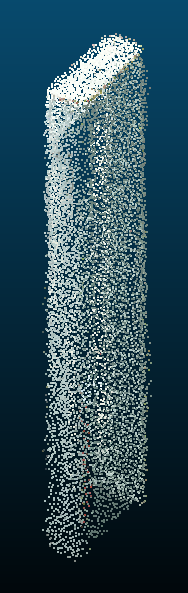
\includegraphics[width=0.52\textwidth]{figures/c4/deep_1_a2.png}
            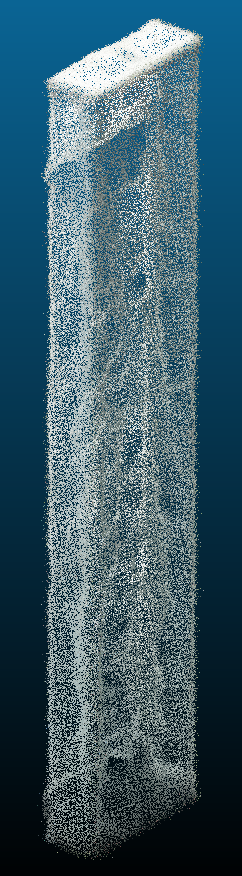
\includegraphics[width=0.45\textwidth]{figures/c4/nerf_deep_1_a2.png}
            \caption{Ăng-ten 1}
        \end{subfigure}
        \hfill
        % Cặp 2
        \begin{subfigure}[b]{0.3\textwidth}
            \centering
            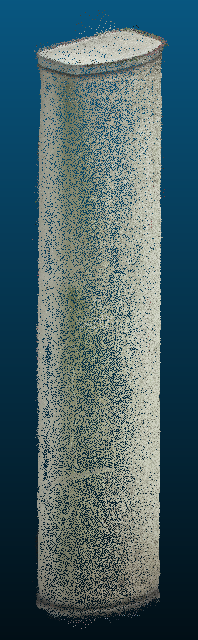
\includegraphics[width=0.5\textwidth]{figures/c4/deep_3_a1.png}
            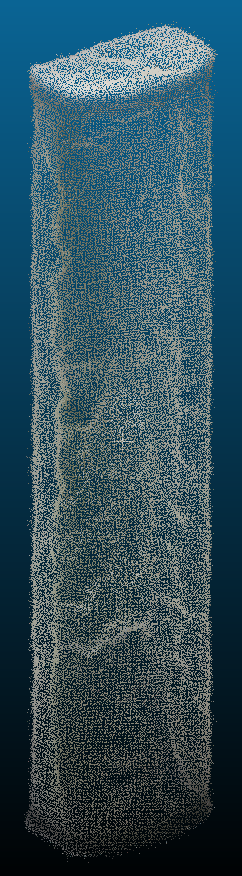
\includegraphics[width=0.445\textwidth]{figures/c4/nerf_deep_3_a1.png}
            \caption{Ăng-ten 2}
        \end{subfigure}
        \hfill
        % Cặp 3
        \begin{subfigure}[b]{0.3\textwidth}
            \centering
            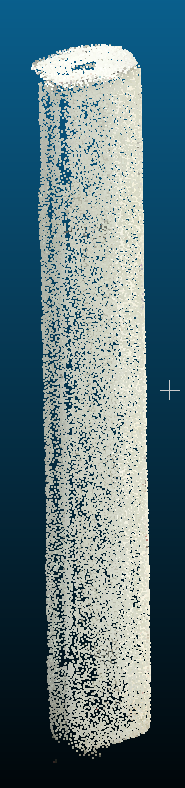
\includegraphics[width=0.375\textwidth]{figures/c4/deep_5_a1.png}
            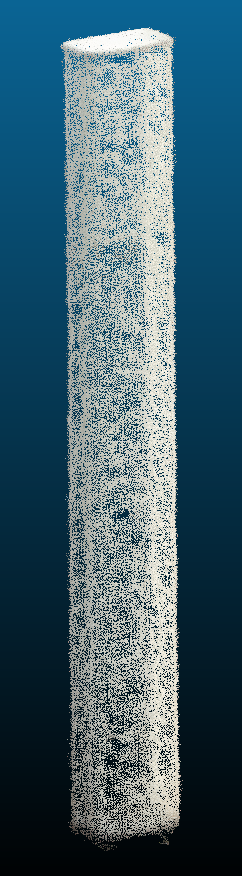
\includegraphics[width=0.44\textwidth]{figures/c4/nerf_deep_5_a1.png}
            \caption{Ăng-ten 3}
        \end{subfigure}
    
        \caption{So sánh biểu diễn mây điểm 3D của các thiết bị ăng-ten được tái tạo bằng MVS (bên trái) và Nerfacto (bên phải) với đầu vào từ SIFT-8K+ALIKED-8K+NF.}
        \label{fig:mvs_nerf_device}
    \end{figure}
    
    Chúng tôi thực hiện so sánh chất lượng mô hình đám mây điểm 3D được tái tạo từ MVS và NeRF  với camera pose tốt nhất được lựa chọn ở trên là SIFT-8K+ALIKED-8K+NF và đánh giá trên 3 tập dữ liệu BTS01, BTS03, BTS05. Hình \ref{fig:3d_mvs_nerf_bts01}, Hình \ref{fig:3d_mvs_nerf_bts03} và Hình \ref{fig:3d_mvs_nerf_bts05} mô tả ảnh chụp vùng thiết bị ăng-ten, RRU được lắp đặt trên mỗi cột đã thực hiện qua cùng 1 bước lọc nhiễu ngoại lai dựa trên thống kê. Có thể dễ dàng nhận thấy bằng mắt thường rằng, mức độ chi tiết, độ ổn định của các điểm trên mô hình của phương pháp biến thể Nerfacto cho kết quả tốt hơn vượt trội so với MVS truyền thống. Tuy nhiên, đối với những đối tượng mà MVS có thể tái tạo được, thì độ chính xác hình học của các đối tượng này lại tốt hơn đáng kể so với NeRF. Quan sát Hình \ref{fig:mvs_nerf_device}, ta thấy rằng, bề mặt thiết bị được tái tạo bởi Nerfacto có tình trạng gợn sóng, không bằng phẳng, trong khi đó bề mặt thiết bị được tái tạo bởi MVS lại phẳng, mịn hơn rất nhiều. Điều này cũng được phản ánh thông qua việc chỉ số PCS trong Bảng \ref{tab:Smoothness_comparison_mvs} thấp hơn khá nhiều so với giá trị trong Bảng \ref{tab:Smoothness_comparison_nerf}. 


    \begin{figure}[htbp]
        \centering
    
        % Hàng trên
        \begin{subfigure}[b]{0.36\textwidth}
            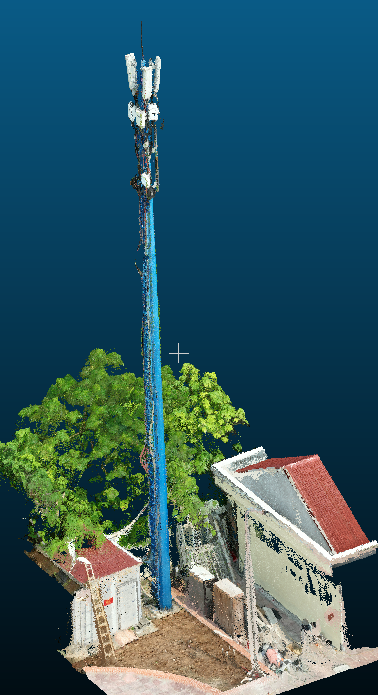
\includegraphics[width=\textwidth]{figures/c4/bts01_mvs_1.png}
        \end{subfigure}
        \hfill
        \begin{subfigure}[b]{0.31\textwidth}
            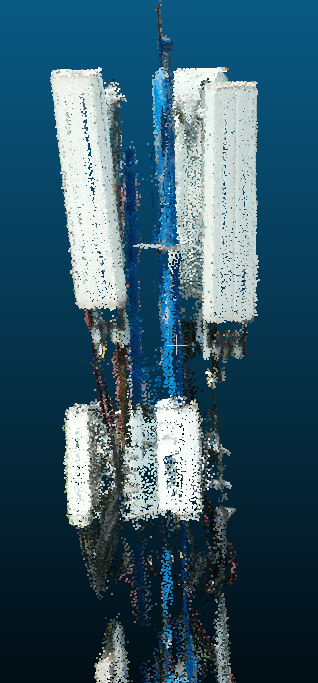
\includegraphics[width=\textwidth]{figures/c4/bts01_mvs_2.png}
        \end{subfigure}
        \hfill
        \begin{subfigure}[b]{0.31\textwidth}
            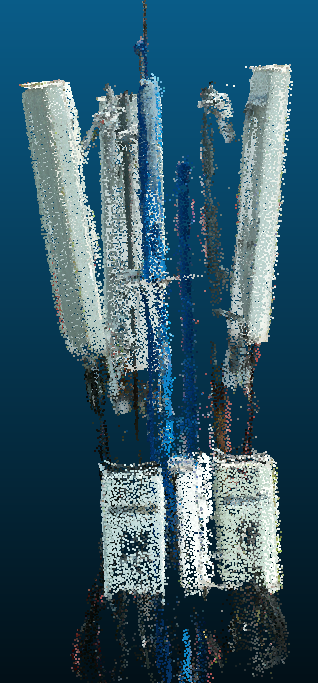
\includegraphics[width=\textwidth]{figures/c4/bts01_mvs_3.png}
        \end{subfigure}
    
        \vspace{0.5cm} % khoảng cách giữa 2 hàng ảnh
    
        % Hàng dưới
        \begin{subfigure}[b]{0.42\textwidth}
            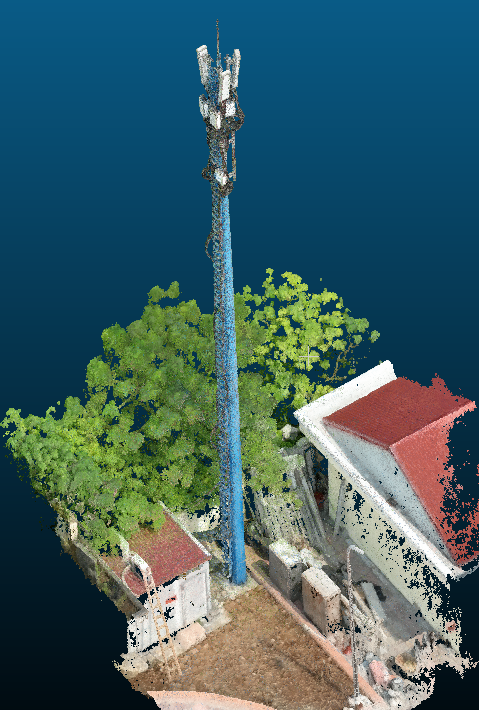
\includegraphics[width=\textwidth]{figures/c4/bts01_nerf_1.png}
          
        \end{subfigure}
        \hfill
        \begin{subfigure}[b]{0.26\textwidth}
            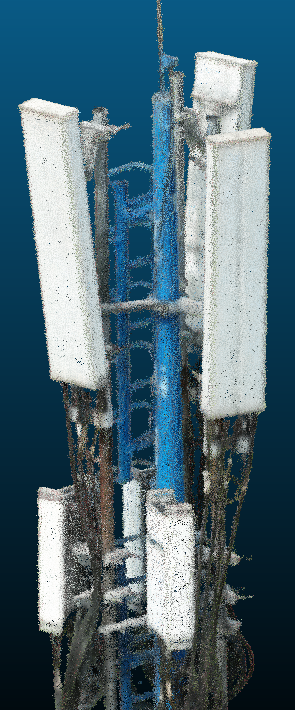
\includegraphics[width=\textwidth]{figures/c4/bts01_nerf_2.png}
            
        \end{subfigure}
        \hfill
        \begin{subfigure}[b]{0.27\textwidth}
            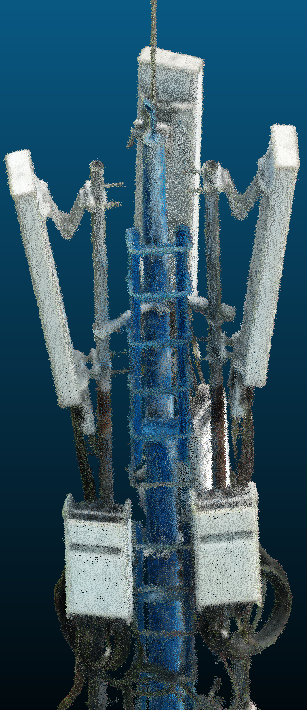
\includegraphics[width=\textwidth]{figures/c4/bts01_nerf_3.png}
           
        \end{subfigure}
    
        \caption{So sánh chất lượng mô hình 3D tái tạo của 2 phương pháp MVS (trên) và Nerfacto (dưới) cho trạm trạm BTS01.}
        \label{fig:3d_mvs_nerf_bts01}
    \end{figure}
     
    \begin{figure}[htbp]
        \centering
    
        % Hàng trên
        \begin{subfigure}[b]{0.28\textwidth}
            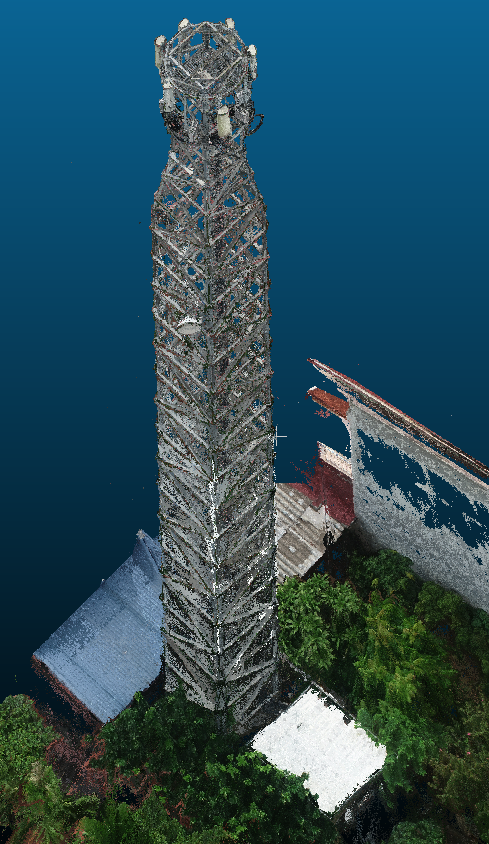
\includegraphics[width=\textwidth]{figures/c4/bts03_mvs_1.png}
        \end{subfigure}
        \hfill
        \begin{subfigure}[b]{0.33\textwidth}
            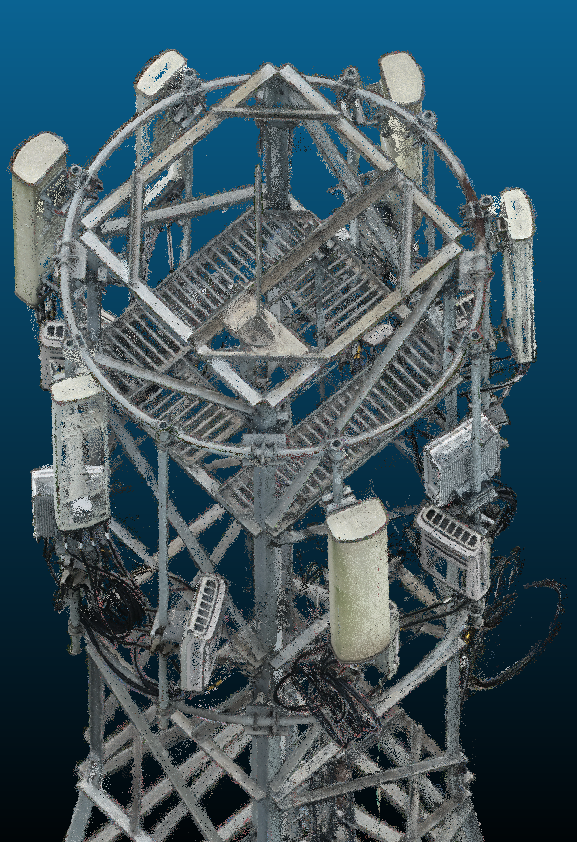
\includegraphics[width=\textwidth]{figures/c4/bts03_mvs_2.png}
        \end{subfigure}
        \hfill
        \begin{subfigure}[b]{0.33\textwidth}
            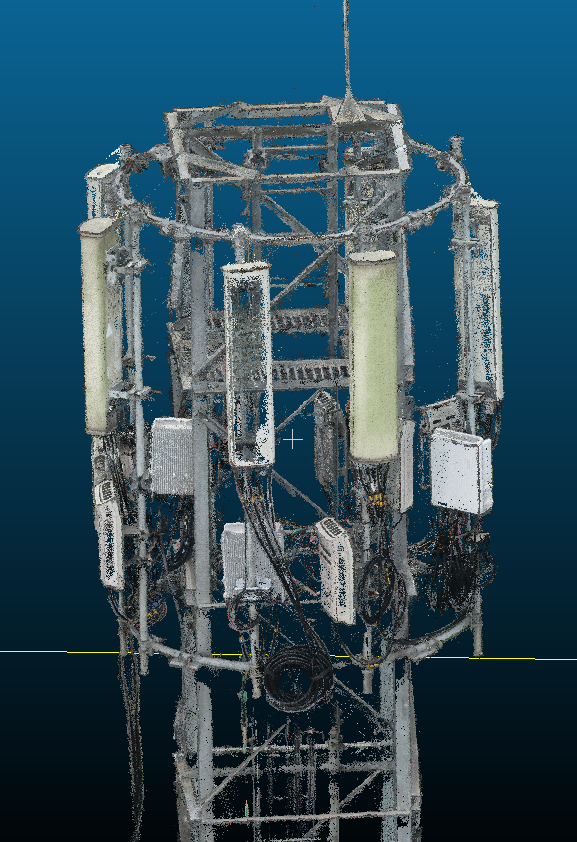
\includegraphics[width=\textwidth]{figures/c4/bts03_mvs_3.png}
        \end{subfigure}
    
        \vspace{0.5cm} % khoảng cách giữa 2 hàng ảnh
    
        % Hàng dưới
        \begin{subfigure}[b]{0.3\textwidth}
            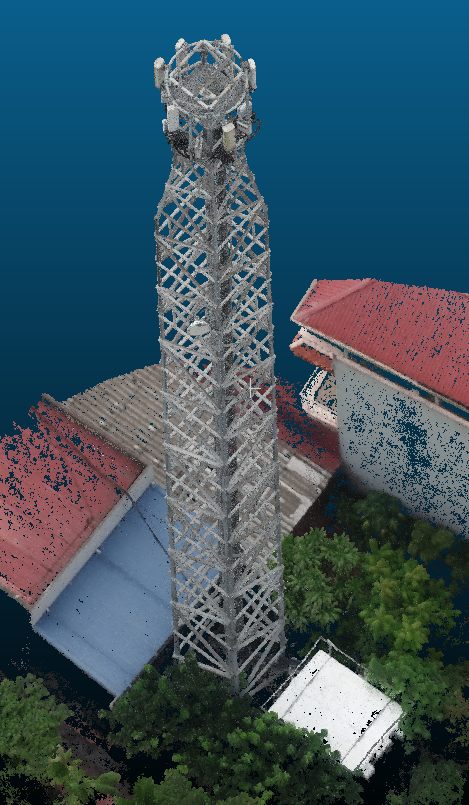
\includegraphics[width=\textwidth]{figures/c4/bts03_nerf_1.png}
          
        \end{subfigure}
        \hfill
        \begin{subfigure}[b]{0.36\textwidth}
            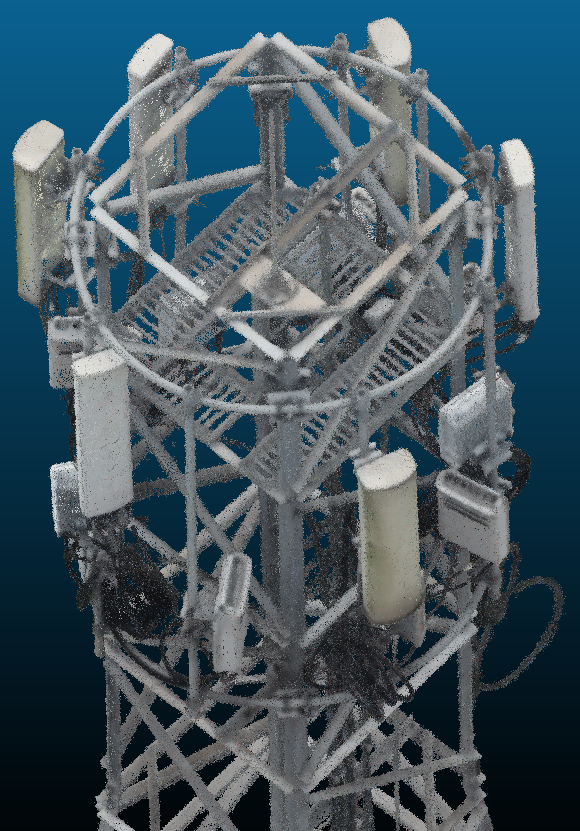
\includegraphics[width=\textwidth]{figures/c4/bts03_nerf_2.png}
            
        \end{subfigure}
        \hfill
        \begin{subfigure}[b]{0.29\textwidth}
            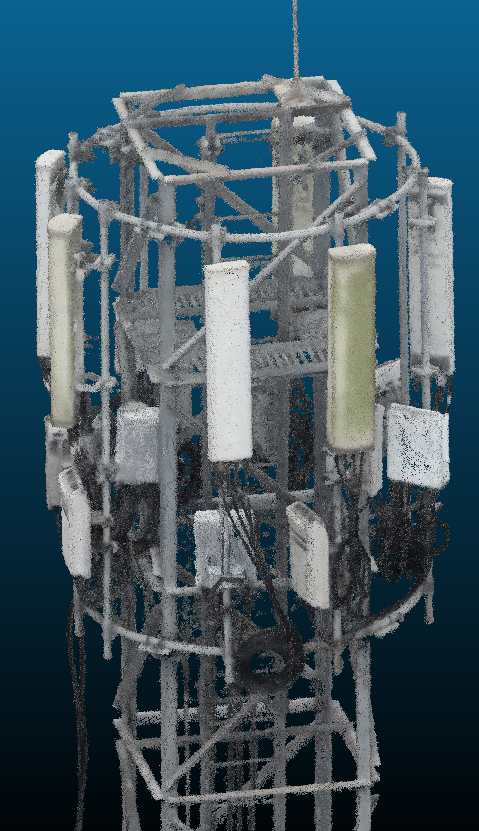
\includegraphics[width=\textwidth]{figures/c4/bts03_nerf_3.png}
           
        \end{subfigure}
    
        \caption{So sánh chất lượng mô hình 3D tái tạo của 2 phương pháp MVS (trên) và Nerfacto (dưới) cho trạm trạm BTS03.}
        \label{fig:3d_mvs_nerf_bts03}
    \end{figure}


    \begin{figure}[htbp]
        \centering
    
        % Hàng trên
        \begin{subfigure}[b]{0.37\textwidth}
            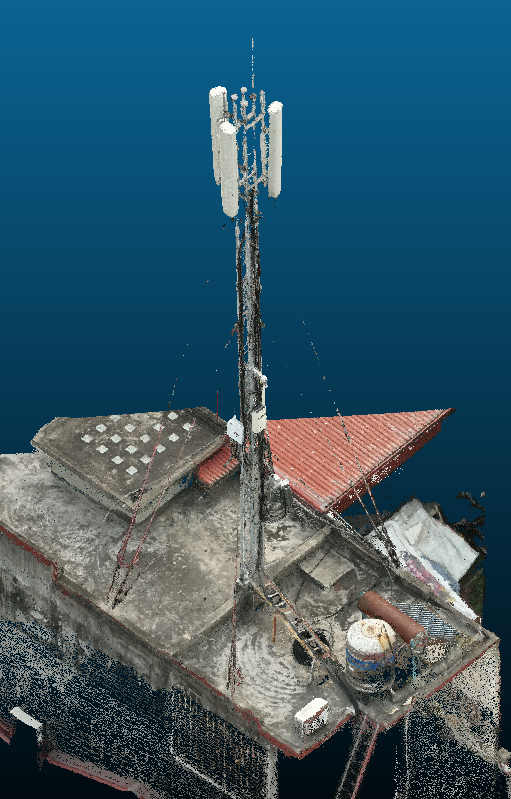
\includegraphics[width=\textwidth]{figures/c4/bts05_mvs_1.png}
        \end{subfigure}
        \hfill
        \begin{subfigure}[b]{0.28\textwidth}
            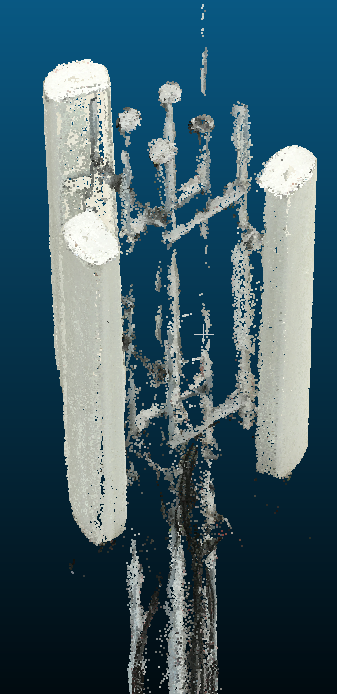
\includegraphics[width=\textwidth]{figures/c4/bts05_mvs_2.png}
        \end{subfigure}
        \hfill
        \begin{subfigure}[b]{0.28\textwidth}
            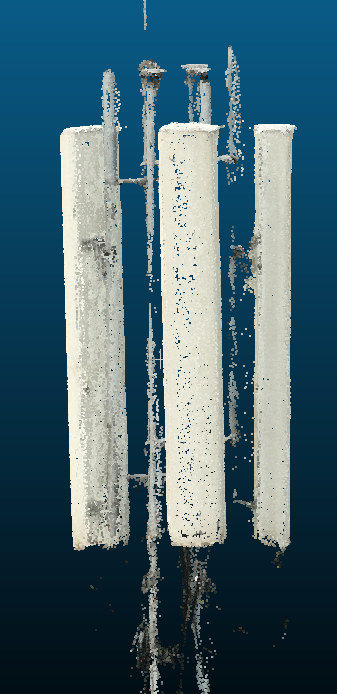
\includegraphics[width=\textwidth]{figures/c4/bts05_mvs_3.png}
        \end{subfigure}
    
        \vspace{0.5cm} % khoảng cách giữa 2 hàng ảnh
    
        % Hàng dưới
        \begin{subfigure}[b]{0.35\textwidth}
            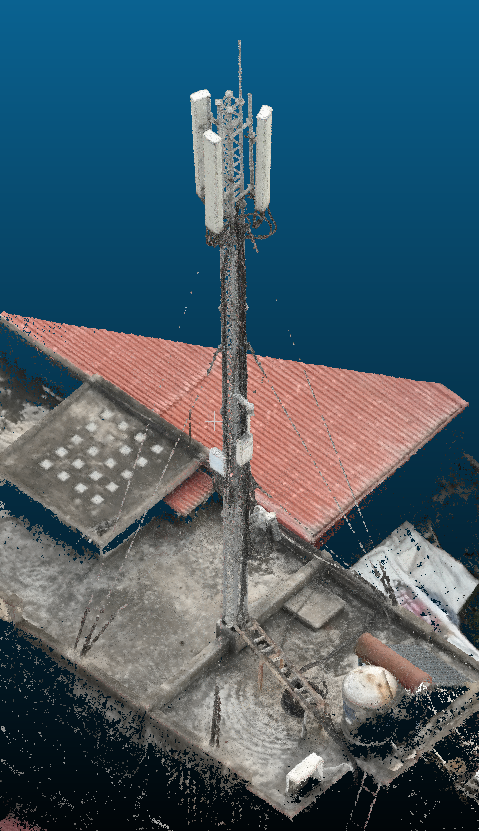
\includegraphics[width=\textwidth]{figures/c4/bts05_nerf_1.png}
          
        \end{subfigure}
        \hfill
        \begin{subfigure}[b]{0.3\textwidth}
            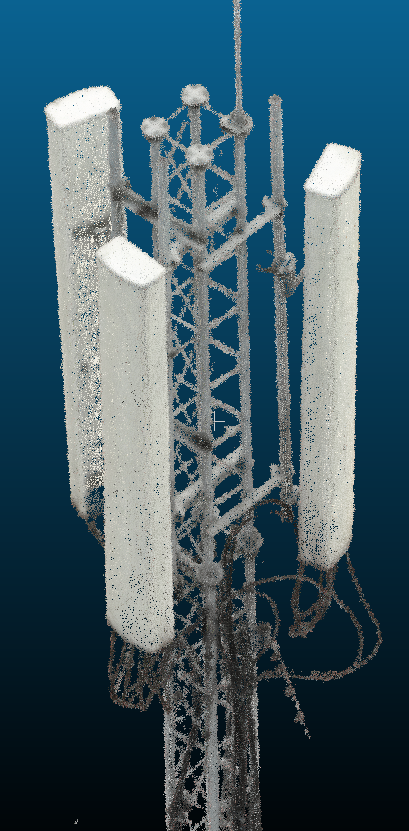
\includegraphics[width=\textwidth]{figures/c4/bts05_nerf_2.png}
            
        \end{subfigure}
        \hfill
        \begin{subfigure}[b]{0.275\textwidth}
            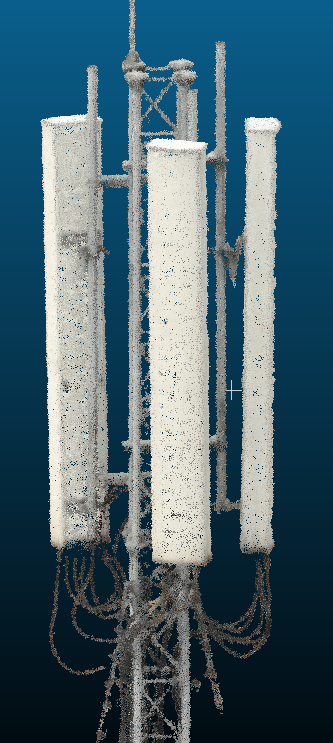
\includegraphics[width=\textwidth]{figures/c4/bts05_nerf_3.png}
           
        \end{subfigure}
    
        \caption{So sánh chất lượng mô hình 3D tái tạo của 2 phương pháp MVS (trên) và Nerfacto (dưới) cho trạm trạm BTS05.}
        \label{fig:3d_mvs_nerf_bts05}
    \end{figure}
    
    % \begin{figure}[H]
    %     \centering
    %     \begin{subfigure}[b]{0.45\textwidth}
    %         \centering
    %         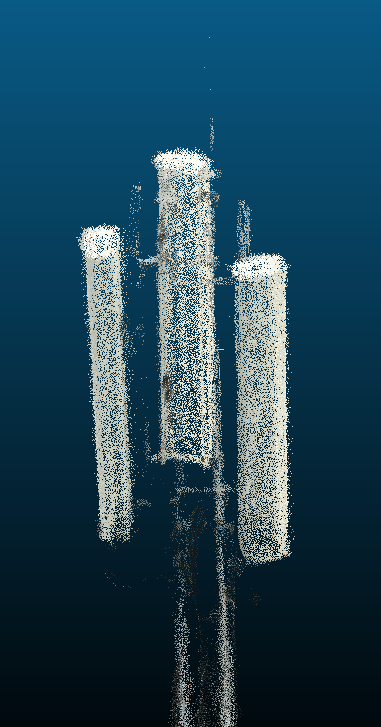
\includegraphics[width=0.85\linewidth]{figures/c4/bts05_mvs.png}
    %         % \caption{Ảnh 1}
    %         \end{subfigure}
    %     \hfill
    %     \begin{subfigure}[b]{0.45\textwidth}
    %         \centering
    %         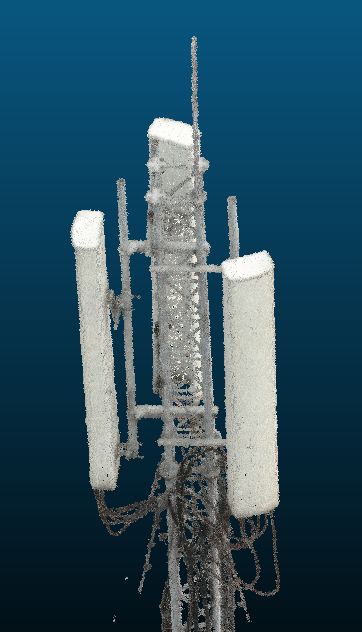
\includegraphics[width=0.85\linewidth]{figures/c4/bts05_nerf.png}
    %         % \caption{Ảnh 2}
    %         \end{subfigure}
    %     \caption{So sánh chất lượng mô hình 3D tái tạo của 2 phương pháp MVS (bên trái) và Nerfacto (bên phải) cho trạm trạm BTS05.}
    %     \label{fig:3d_mvs_nerf_bts05}
    % \end{figure}
        
        
\section{Thảo luận}
\label{sec:discussion}
    \subsection{Phân tích hiệu quả và hạn chế của phương pháp đề xuất}
\label{subsec:discuss_proposed_method}

Thông qua các kết quả thực nghiệm định lượng và định tính được trình bày chi tiết trong Mục \ref{sec:eval_pose}, phương pháp SfM lai ghép đề xuất đã cho thấy hiệu quả rõ rệt trong việc nâng cao độ chính xác ước tính camera pose so với phương pháp SfM truyền thống dựa trên SIFT khi áp dụng cho bộ dữ liệu ảnh chụp cột ăng-ten viễn thông. Các chỉ số như sai số chiếu lại trung bình (MRE) giảm trung bình khoảng 15\% là minh chứng cho sự vượt trội này. 

Sự cải thiện này có thể được lý giải thông qua đóng góp của các thành phần chính trong quy trình đề xuất. Thứ nhất, việc áp dụng phát hiện vùng ảnh cột sử dụng mô hình YOLO-v11 cho phép áp dụng các bộ trích xuất đặc trưng phù hợp với từng vùng ảnh. Cụ thể, ALIKED và LightGlue đã phát huy hiệu quả trên vùng tập trung của cột vốn có bề mặt trơn, thiếu vân đặc trưng. Đồng thời, việc vẫn ưu tiên kết hợp sử dụng SIFT giúp duy trì các điểm đặc trưng có tính bất biến, đáng tin cậy. Thứ hai, bước lọc các điểm đặc trưng dựa trên độ sâu tương đối ước tính từ Depth Anything V2 đã chứng minh vai trò quan trọng trong việc loại bỏ các đăc trưng nhiễu, không đáng tin cậy ở hậu cảnh xa. Việc loại bỏ các điểm này giúp ổn định quá trình Tối ưu hình học, tránh các lỗi tối ưu hóa do các điểm ở xa hoặc gần vô cực gây ra, từ đó cải thiện độ chính xác và tính nhất quán toàn cục của máy ảnh cuối cùng.

Tuy nhiên, phương pháp đề xuất cũng bộc lộ một số hạn chế cần được xem xét. Độ chính xác của kết quả cuối cùng phụ thuộc vào độ chính xác của 2 mô hình học sâu khác nhau là phát hiện vùng cột và ước lượng độ sâu tương đối. Nếu các mô hình này hoạt động không tốt hoàn toàn có thể tạo ra các điểm đặc trưng nhiễu ảnh hưởng tới các giai đoạn tính toán sau đó. Bên cạnh đó, việc phải thực hiện các bước xử lý với mô hình học sâu có thể làm tăng thời gian xử lý của cả quy trình lên nhiều lần, điều này có thể ảnh hưởng tới khả năng ứng dụng thực tế của giải pháp. Cuối cùng, phương pháp vẫn có thể gặp khó khăn nếu vùng hậu cảnh quá đơn điệu hoặc có tính động lớn (ví dụ xung quanh nhiều cây cối và chụp trong điều kiện có gió) hoặc các vùng có tính lặp lại quá cao, khó phân biệt như trên rừng cây,... từ đó làm giảm chất lượng của các đặc trưng SIFT dùng để định vị toàn cục.

\subsection{Phân tích hiệu quả MVS và NeRF cho cột ăng-ten}
\label{subsec:discuss_mvs_nerf}

Sau khi thu được camera pose có độ chính xác cao từ phương pháp SfM lai ghép đề xuất, luận văn đã tiến hành đánh giá hai phương pháp tái tạo đám mây điểm 3D dày đặc phổ biến là MVS (sử dụng COLMAP MVS) và NeRF (sử dụng biến thể nerfacto) cho đối tượng đặc thù là cột ăng-ten viễn thông. Kết quả thực nghiệm tại Mục \ref{sec:eval_dense} cung cấp những phân tích so sánh giá trị về ưu và nhược điểm của từng phương pháp trong bối cảnh ứng dụng này.

Kết quả cho thấy, mô hình NeRF (cụ thể là nerfacto) tỏ ra vượt trội hơn MVS về một số khía cạnh quan trọng. Thứ nhất, NeRF tạo ra mô hình 3D có chất lượng tổng thể tốt hơn, mật độ điểm cao và độ bao phủ bề mặt đầy đủ hơn đáng kể so với MVS. Đặc biệt, NeRF đã giải quyết được một trong những thách thức lớn nhất của MVS truyền thống là tái tạo các bề mặt thiết bị trơn nhẵn, thiếu vân đặc trưng (vỏ nhựa/composite của ăng-ten, RRU); mô hình NeRF không bị hiện tượng thủng lỗ các vùng này như thường thấy ở kết quả của MVS. Khả năng này đến từ bản chất của NeRF là học một biểu diễn nơ-ron cho không gian liên tục và tối ưu hóa dựa trên hàm lỗi quang học trên toàn bộ tia nhìn, thay vì phụ thuộc vào việc khớp nối các vùng ảnh cục bộ như MVS.

Tuy nhiên, mô hình 3D được trích xuất từ NeRF cũng bộc lộ hạn chế về độ mượt và độ chính xác hình học cục bộ của bề mặt đối tượng (nhà, thiết bị, thân cột). Kết quả cho thấy bề mặt tái tạo từ NeRF có xu hướng bị "gợn sóng" hoặc thiếu độ phẳng cần thiết, đặc biệt là trên các bề mặt lớn. Ngược lại, MVS, mặc dù thất bại trong việc tái tạo các vùng thiếu đặc trưng, lại thể hiện khả năng đảm bảo cấu trúc hình học tốt hơn và tạo ra các bề mặt phẳng, các cạnh sắc nét hơn tại những vùng mà nó có thể tái tạo được. Điều này là bởi MVS dựa trên các ràng buộc hình học rõ ràng hơn trong quá trình ước tính độ sâu cục bộ.

Xét về khả năng ứng dụng, mặc dù bề mặt tái tạo từ NeRF chưa hoàn toàn phẳng mịn, nhưng độ đầy đủ và khả năng bao phủ toàn bộ thiết bị của nó lại là một lợi thế lớn. Như kết quả quan sát được, mô hình NeRF hoàn toàn có thể được sử dụng hiệu quả cho các tác vụ mở rộng dựa trên mô hình 3D như tự động phát hiện, nhận diện và tính toán các thông số kỹ thuật của thiết bị vô tuyến gắn trên cột. Việc có một biểu diễn 3D hoàn chỉnh của thiết bị, ngay cả khi có chút gợn sóng bề mặt, vẫn tốt hơn là một mô hình bị thủng lỗ hoặc thiếu dữ liệu như MVS truyền thống trong việc nhận dạng và đo đạc.

Tóm lại, đối với bài toán tái tạo 3D cột ăng-ten viễn thông, NeRF (cụ thể là biến thể nerfacto) cho thấy tính khả thi thực tế vượt trội so với MVS truyền thống về độ hoàn chỉnh và khả năng xử lý bề mặt khó, rất phù hợp cho các ứng dụng phân tích thiết bị tự động sau này, mặc dù cần cải thiện thêm về độ chính xác yếu tố hình học. MVS vẫn có giá trị ở những vùng có thể tái tạo tốt nếu yêu cầu độ chính xác hình học cục bộ là ưu tiên hàng đầu. Do đó, việc lựa chọn phương pháp tái tạo dày đặc cuối cùng nên dựa trên yêu cầu cụ thể của từng mục tiêu ứng dụng.

\section*{Kết luận Chương 4}
\addcontentsline{toc}{section}{Kết luận Chương 4}
Như vậy, Chương 4 đã trình bày chi tiết các khía cạnh liên quan tới thực nghiệm của luận văn, bao gồm: mô tả dữ liệu, môi trường cài đặt, độ đo đánh giá. Điểm quan trọng là Chương 4 đã đưa ra những thử nghiệm, so sánh, đánh giá chi tiết để kiểm chứng độ hiệu quả của phương pháp đề xuất thông qua so sánh các chỉ số đánh giá rõ ràng. Bên cạnh đó, Chương 4 cũng đánh giá, so sánh sự ảnh hưởng của độ chính xác camera pose tới chất lượng mô hình 3D tái tạo trên 2 phương pháp MVS và NeRF. Từ đó, chúng tôi đưa ra những nhận xét quan trọng về ưu điểm, nhược điểm và tính ứng dụng của mỗi phương pháp.